\section{Systematics}
\label{sec:syst}
The fit's main goal is to minimise impact of systematic parameters for T2K-SK oscillation analyses by using near-detector data. The shared parameters between ND280 and SK are the neutrino flux parameters (since T2K and SK are in the same neutrino ``beamline''), and neutrino-nucleus interaction parameters. The ``nuisance parameters'' can be considered as the ND280 detector parameters and cross-section parameters that are parametrised as only effective on Carbon. As such, there are many ``parameters of interest'', which the following section covers.

The sources of systematics enter the fit by changing the prediction by shape and/or normalisation, and in most cases the fit incurs a likelihood penalty for moving parameters away from their priors. The penalty takes two forms: either Gaussian or a constant. In the case where there is firm reason to believe a parameter is constrained from other sources, the Gaussian penalty is imposed. When external data or recent model development and similar indicate lacking or conflicting knowledge of a parameter, a flat prior is chosen.

For the Gaussian penalty we have
\begin{equation}
	-2\log\mathcal{L}_\text{Penalty} = (X_i-\mu_i) \left(\mathbf{V}_{i,j}\right)^{-1} (X_j-\mu_j)
\end{equation}
for parameter $i$, with current fit values $X_i$, priors $\mu_i$ and covariance matrix $\mathbf{V}$, and for a flat penalty we have
\begin{equation}
	-2\log\mathcal{L}_\text{Penalty} = C
\end{equation}
where $C$ is a constant.

\subsection{Flux}
\label{subsec:syst_flux}
The flux systematics contain uncertainties from all sources going into the neutrino flux prediction. They are primarily split into six categories:
\begin{itemize}
	\item Hadron interaction uncertainties
	\item Proton beam profile and off-axis angle
	\item Horn current and field
	\item Horn and target alignment
	\item Materials modelling
	\item Number of protons on target
\end{itemize}

The software suite for the beam simulation consists of FLUKA2011 \cite{fluka2008_1, fluka2008_2, fluka2011} which simulates hadronic interactions in target and baffle, JNUBEAM (GEANT3-based \cite{geant3}) which simulates the geometry and tracking, and GCALOR \cite{gcalor} which simulates hadronic re-interactions and is used as a cross-check for FLUKA. Full details are found elsewhere \cite{t2k_beam, t2k_tn_flux}.

The simulations are updated each year to improve the modelling, often taking additional data in to account. An example of such is using the dedicated NA61/SHINE T2K replica target data \cite{NA61_pions_rep} to tune the hadron production model at the T2K beam target, and including results from the HARP experiment \cite{harp}.

The effects on the fractional error for the ND280 neutrino flux prediction is shown in \autoref{fig:flux_uncert_fhc} for FHC running and \autoref{fig:flux_uncert_rhc} for RHC running. The uncertainties are $\sim10\%$ in the flux peak region and is dominated by the hadron interaction uncertainties, which in turn consists primarily of multiplicity, pion rescattering and interaction length uncertainties. The proton beam profile and off-axis angle become important shortly after the flux peak at about 1 GeV for the right-sign component of the flux.

\begin{figure}[h]
	\begin{subfigure}[t]{0.42\textwidth}
		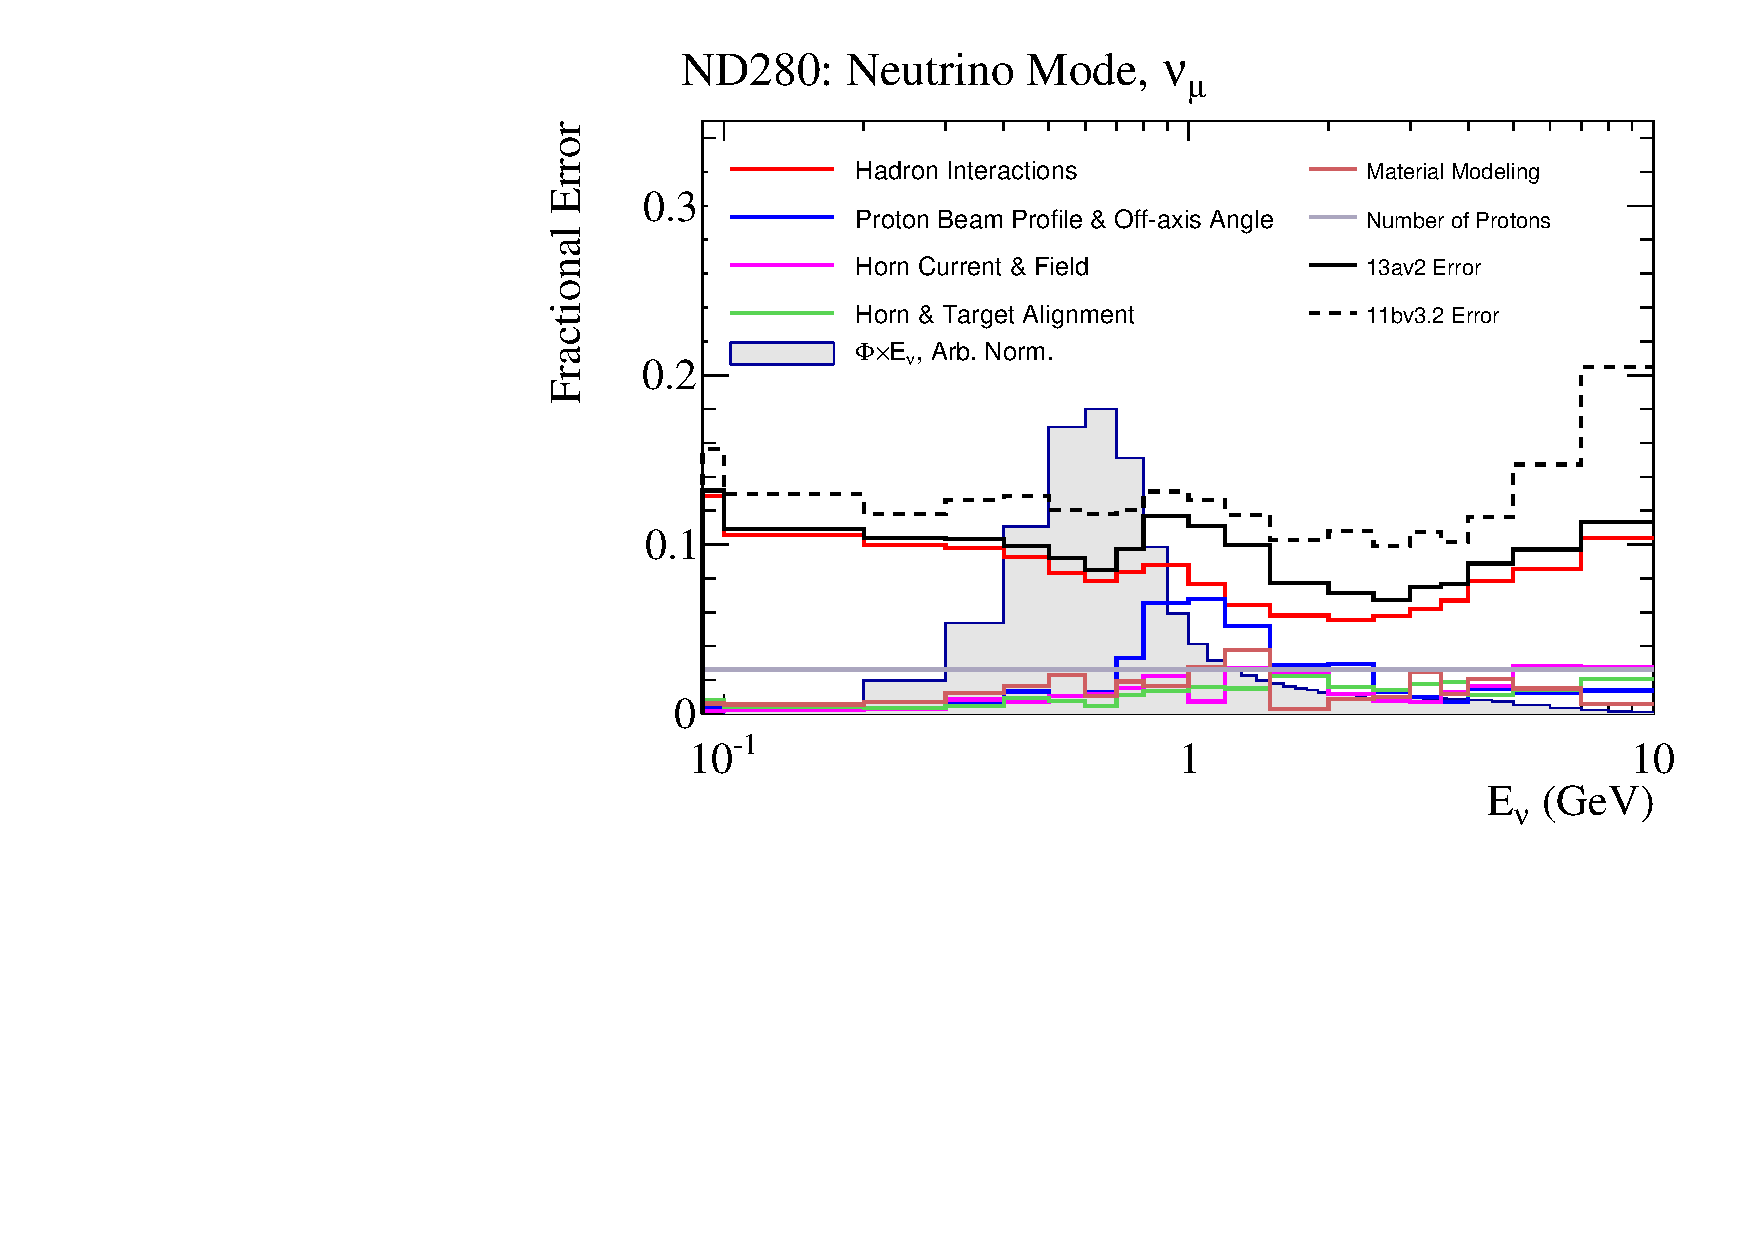
\includegraphics[width=\textwidth, trim={0mm 0mm 0mm 0mm}, clip,page=1]{figures/flux/total_err_nd5_numode_numu}
	\end{subfigure}
	\begin{subfigure}[t]{0.42\textwidth}
		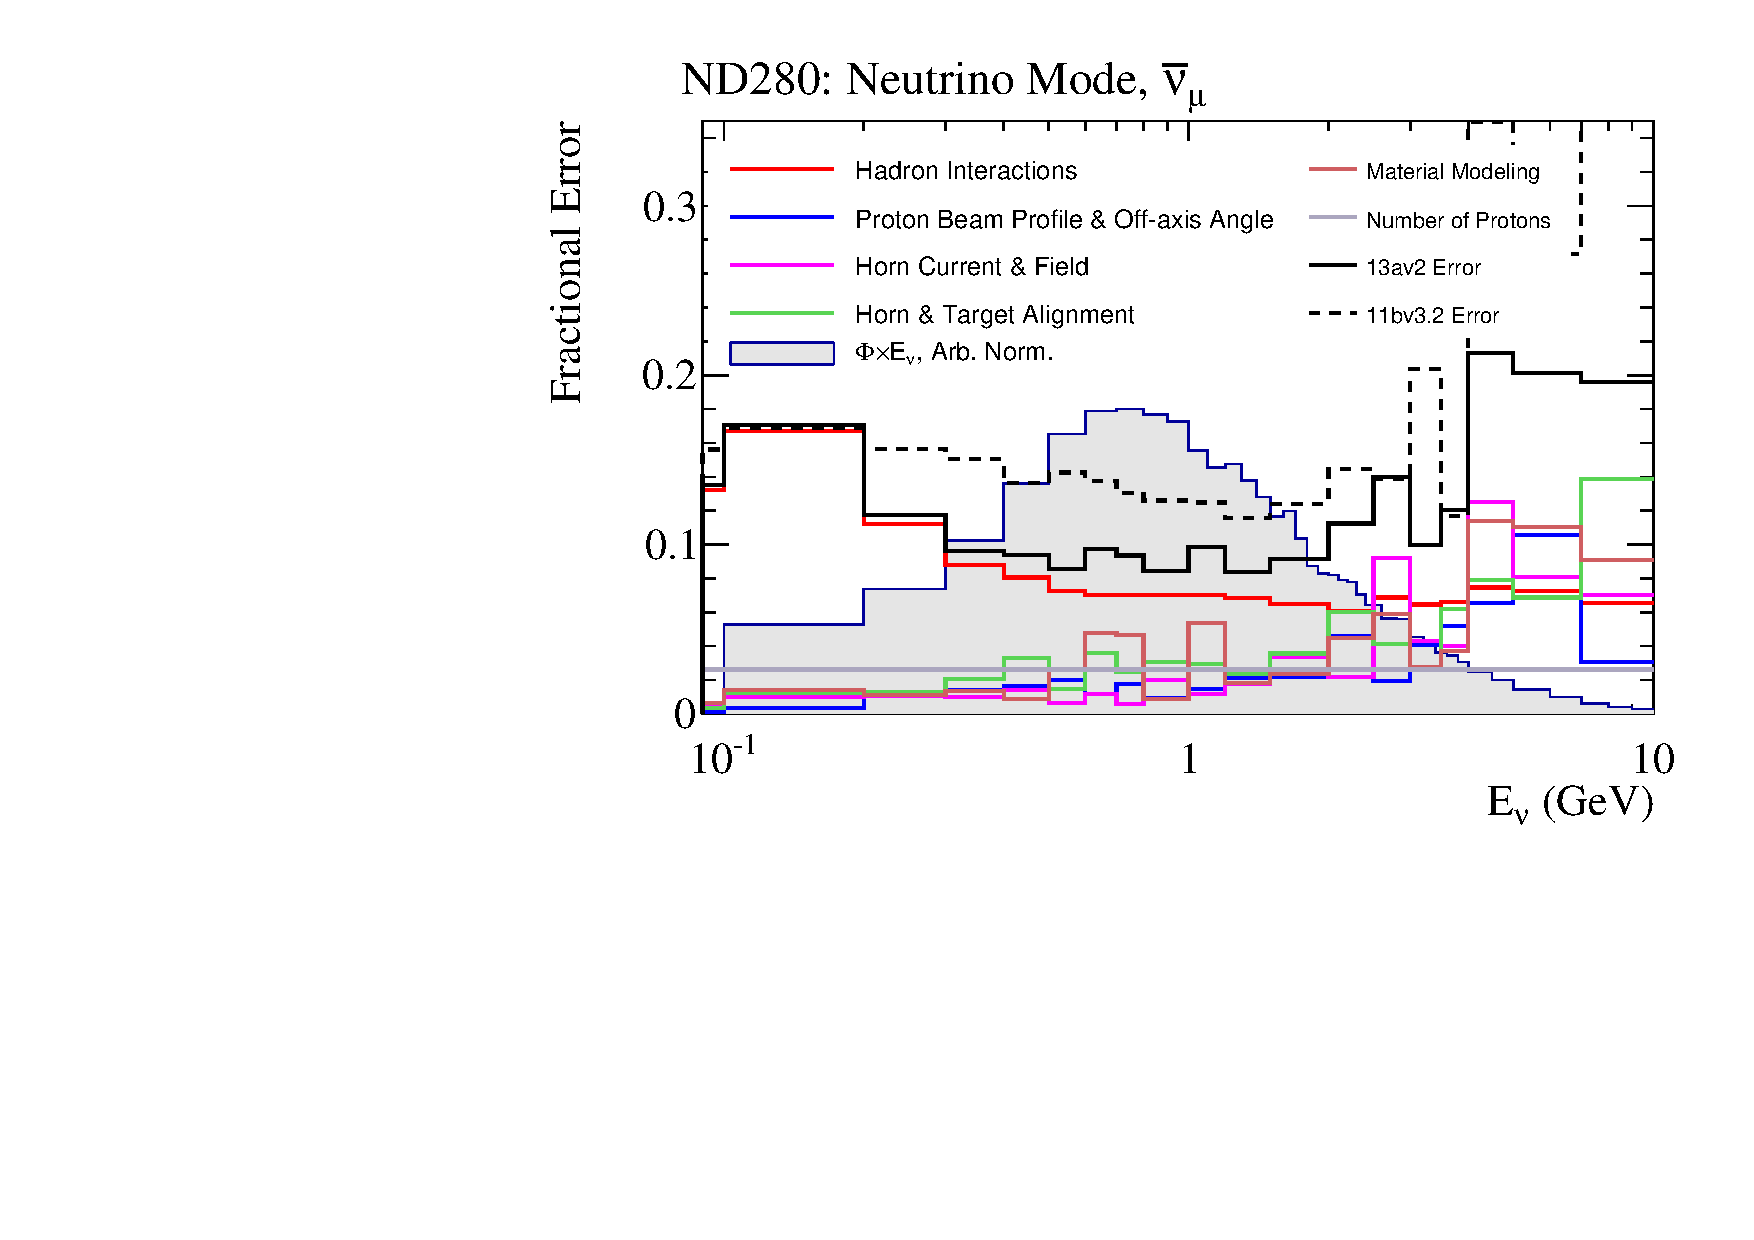
\includegraphics[width=\textwidth, trim={0mm 0mm 0mm 0mm}, clip,page=1]{figures/flux/total_err_nd5_numode_numub}
	\end{subfigure}

	\begin{subfigure}[t]{0.42\textwidth}
		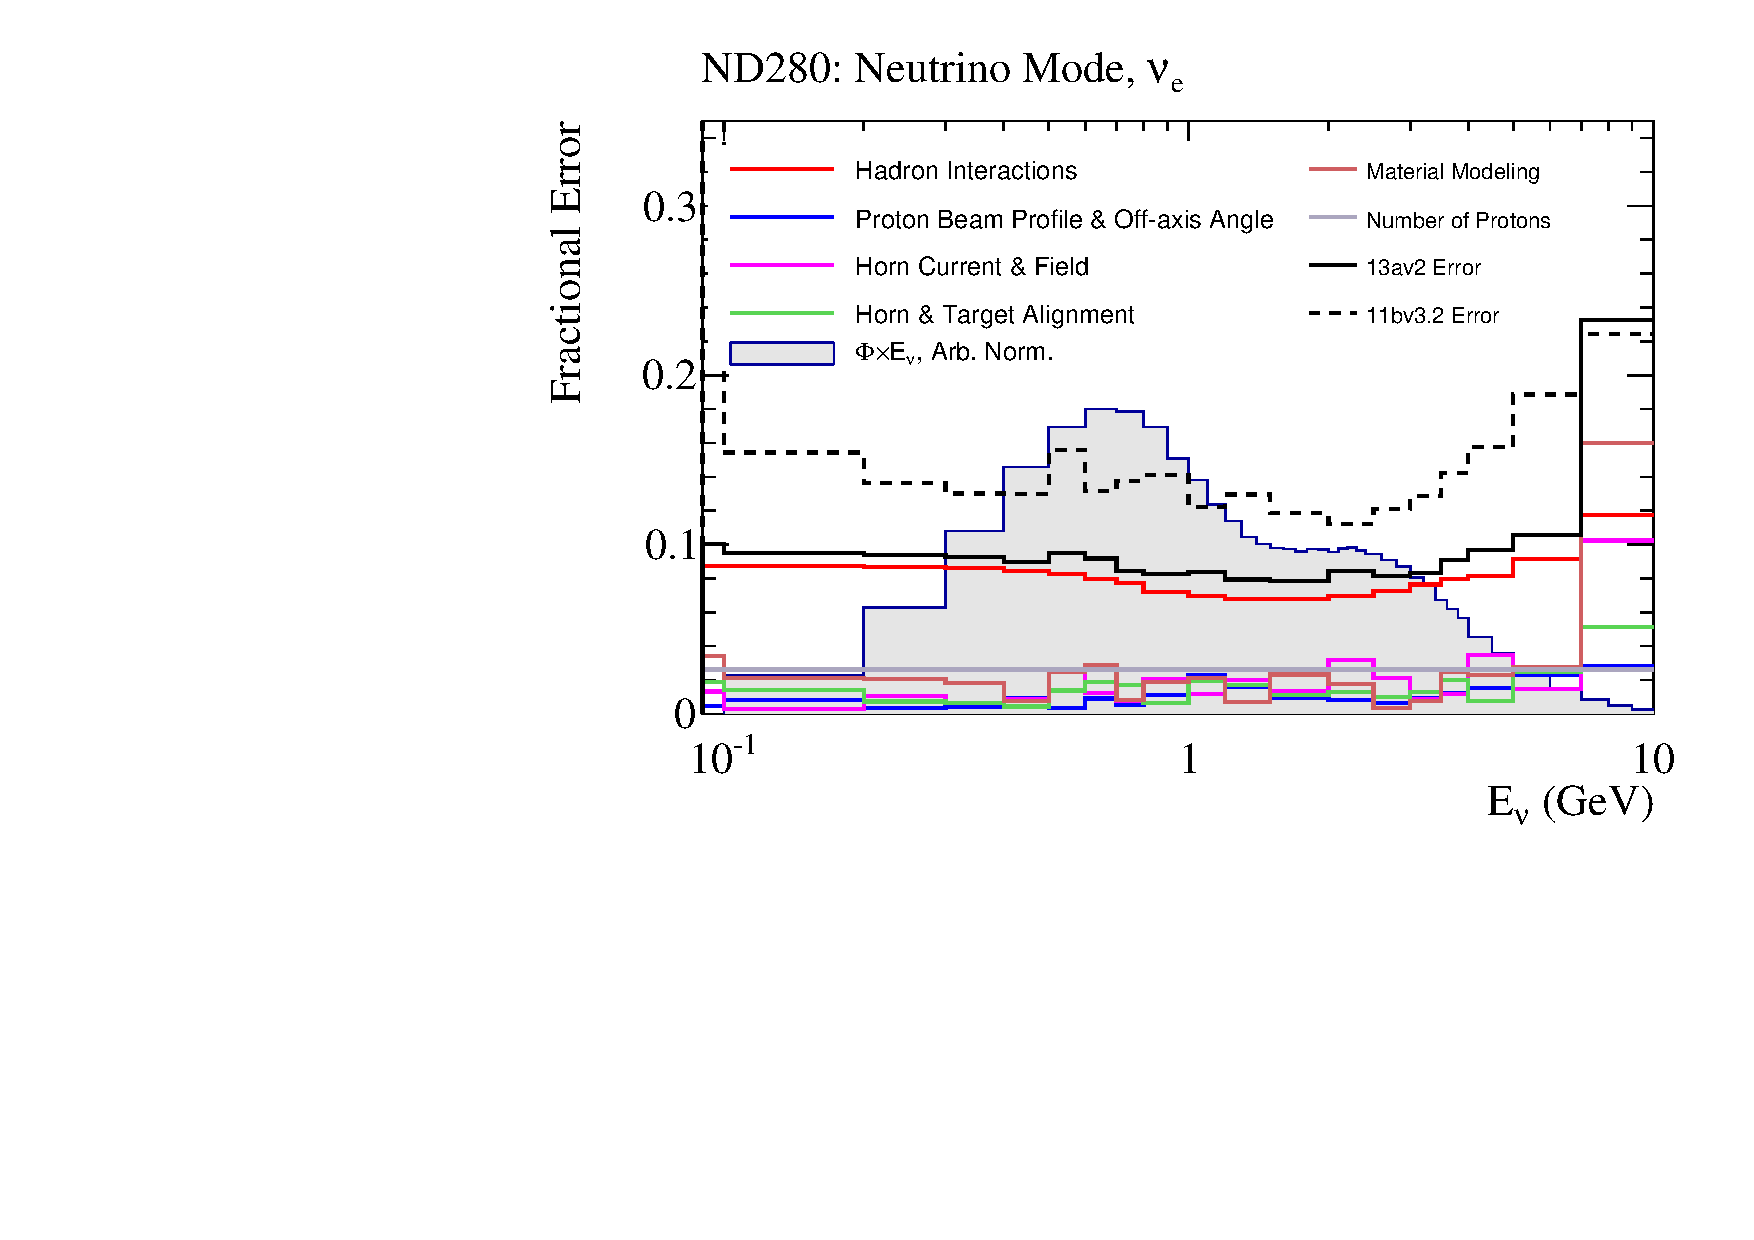
\includegraphics[width=\textwidth, trim={0mm 0mm 0mm 0mm}, clip,page=1]{figures/flux/total_err_nd5_numode_nue}
	\end{subfigure}
	\begin{subfigure}[t]{0.42\textwidth}
		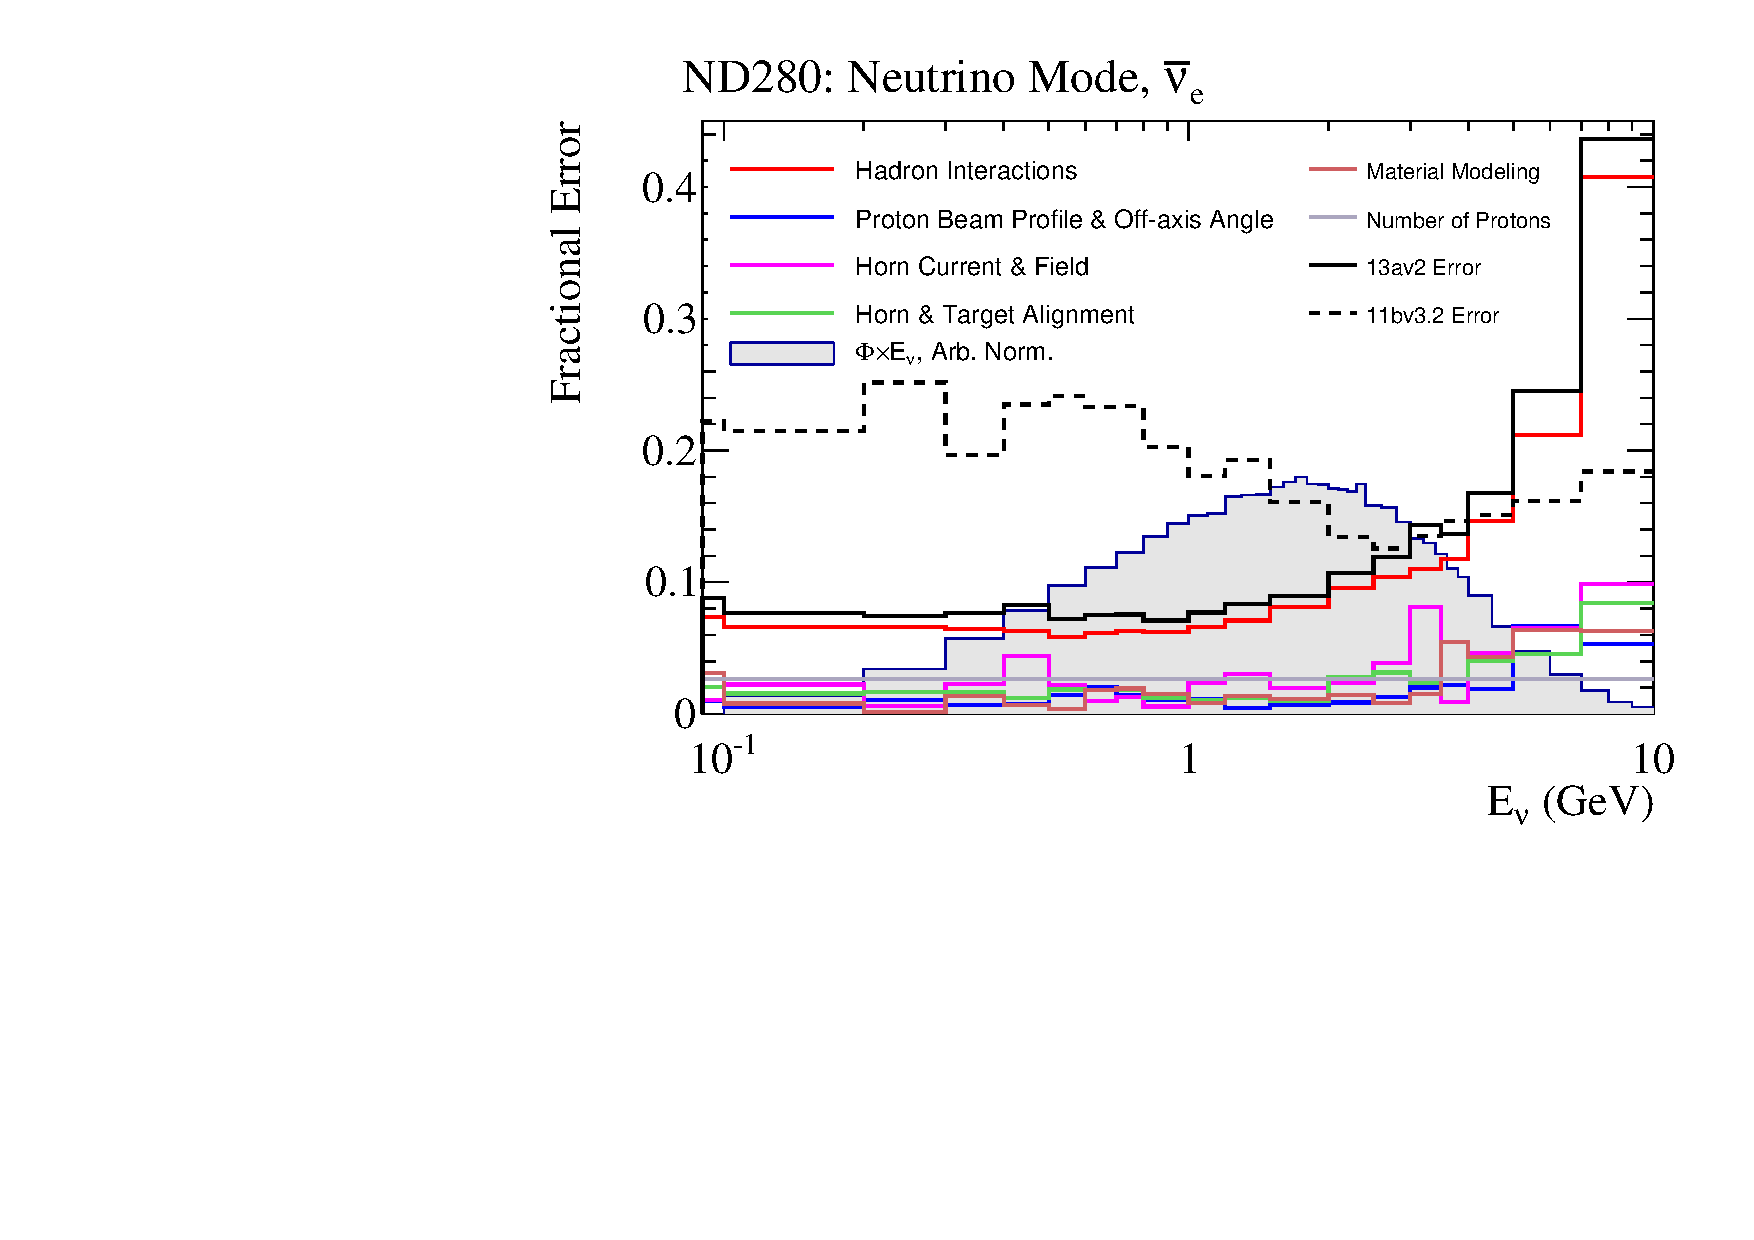
\includegraphics[width=\textwidth, trim={0mm 0mm 0mm 0mm}, clip,page=1]{figures/flux/total_err_nd5_numode_nueb}
	\end{subfigure}
	\caption{FHC flux uncertainties, ``13av2 Error'' is used for this analysis}
	\label{fig:flux_uncert_fhc}
\end{figure}

\begin{figure}[h]
	\begin{subfigure}[t]{0.42\textwidth}
		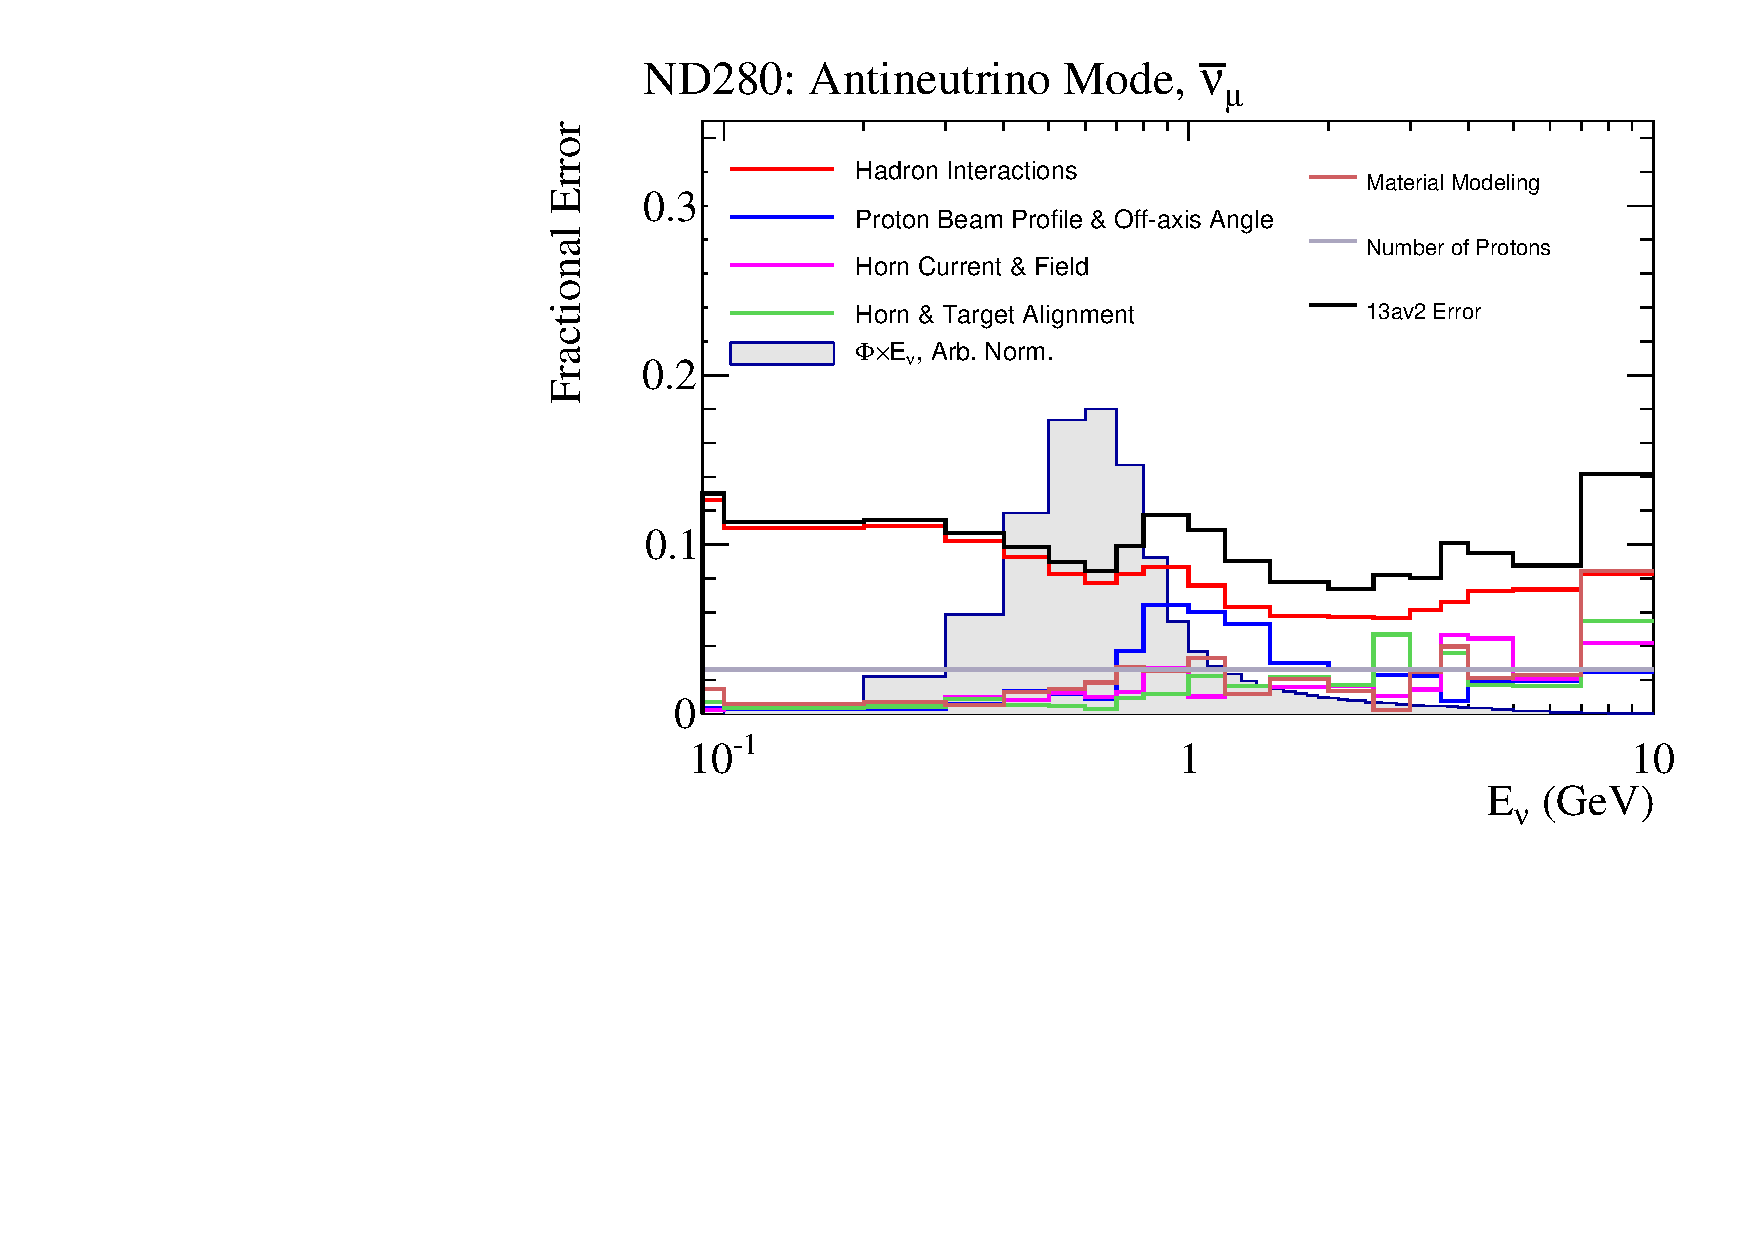
\includegraphics[width=\textwidth, trim={0mm 0mm 0mm 0mm}, clip,page=1]{figures/flux/total_err_nd5_anumode_numub}
	\end{subfigure}
	\begin{subfigure}[t]{0.42\textwidth}
		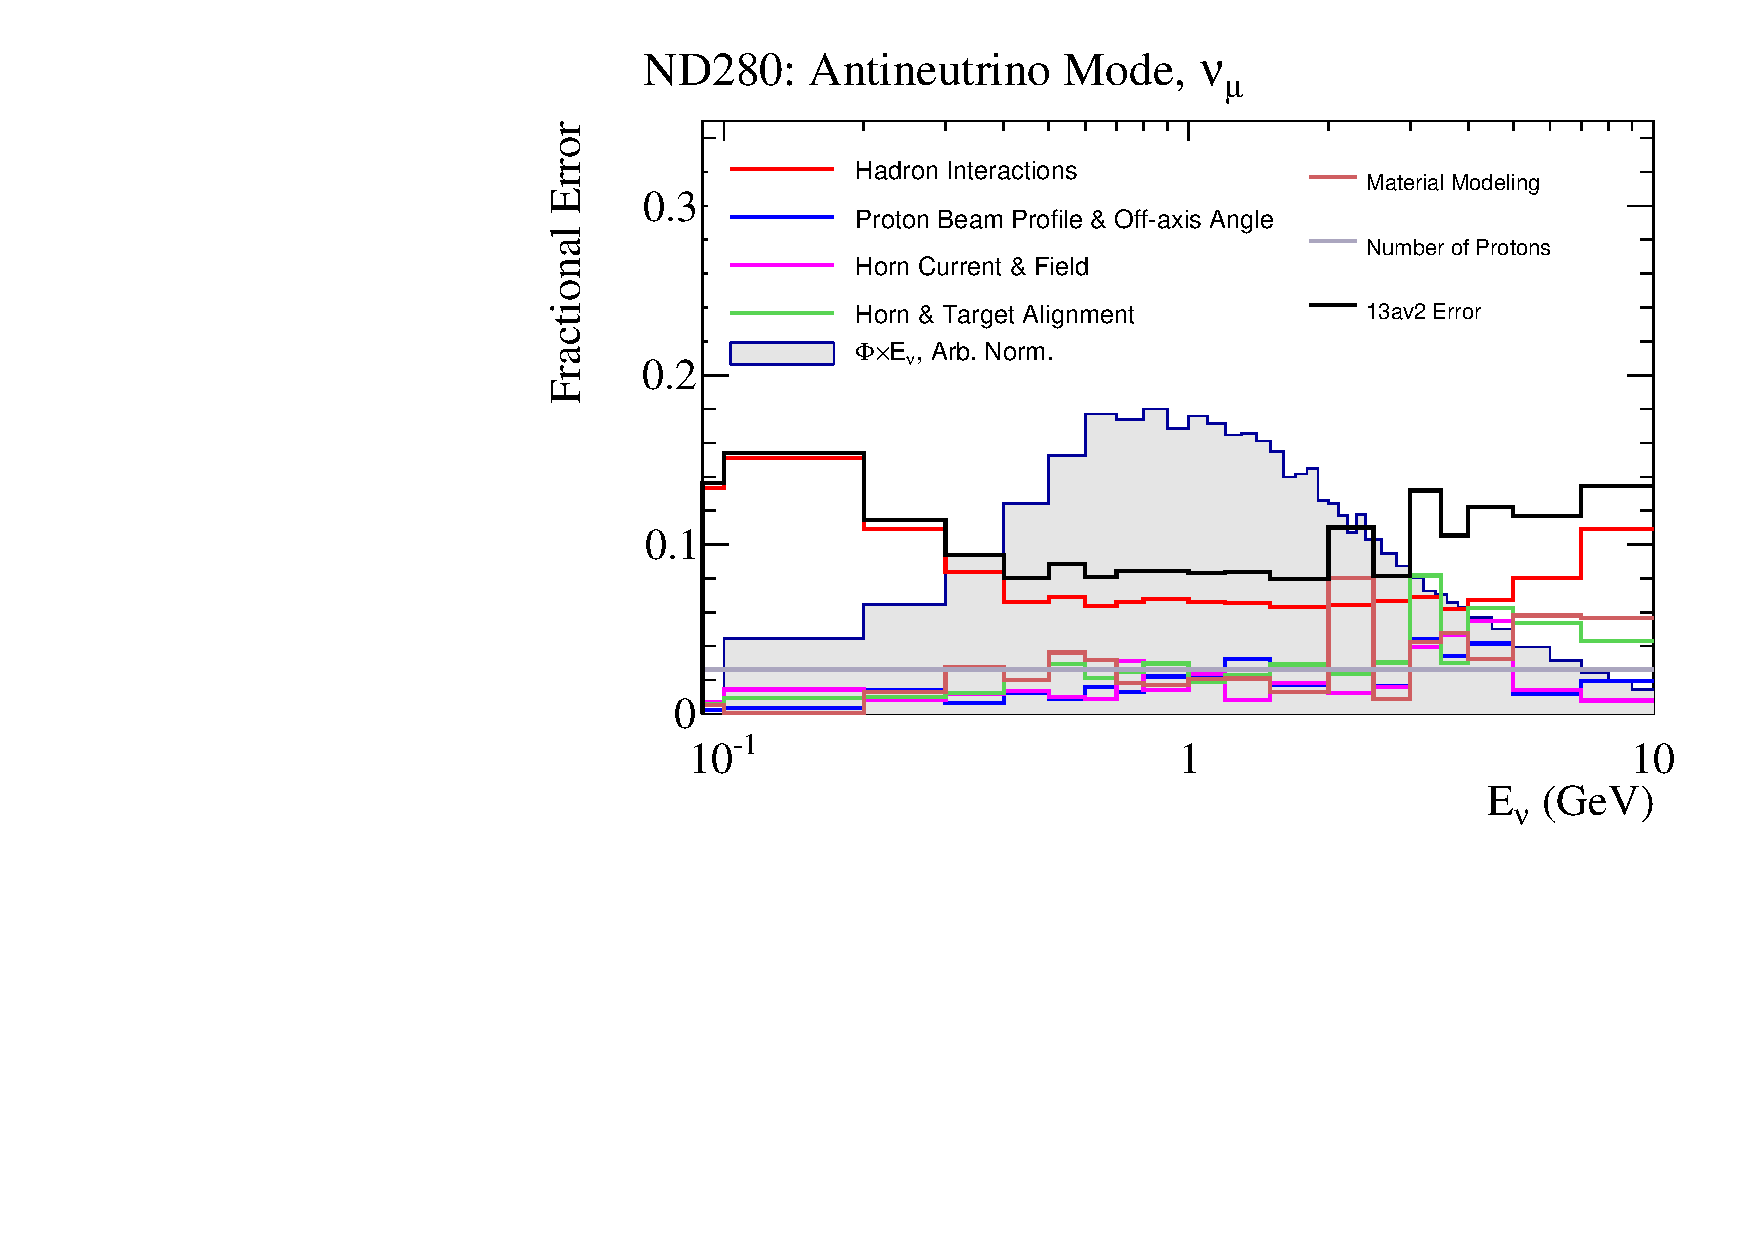
\includegraphics[width=\textwidth, trim={0mm 0mm 0mm 0mm}, clip,page=1]{figures/flux/total_err_nd5_anumode_numu}
	\end{subfigure}

	\begin{subfigure}[t]{0.42\textwidth}
		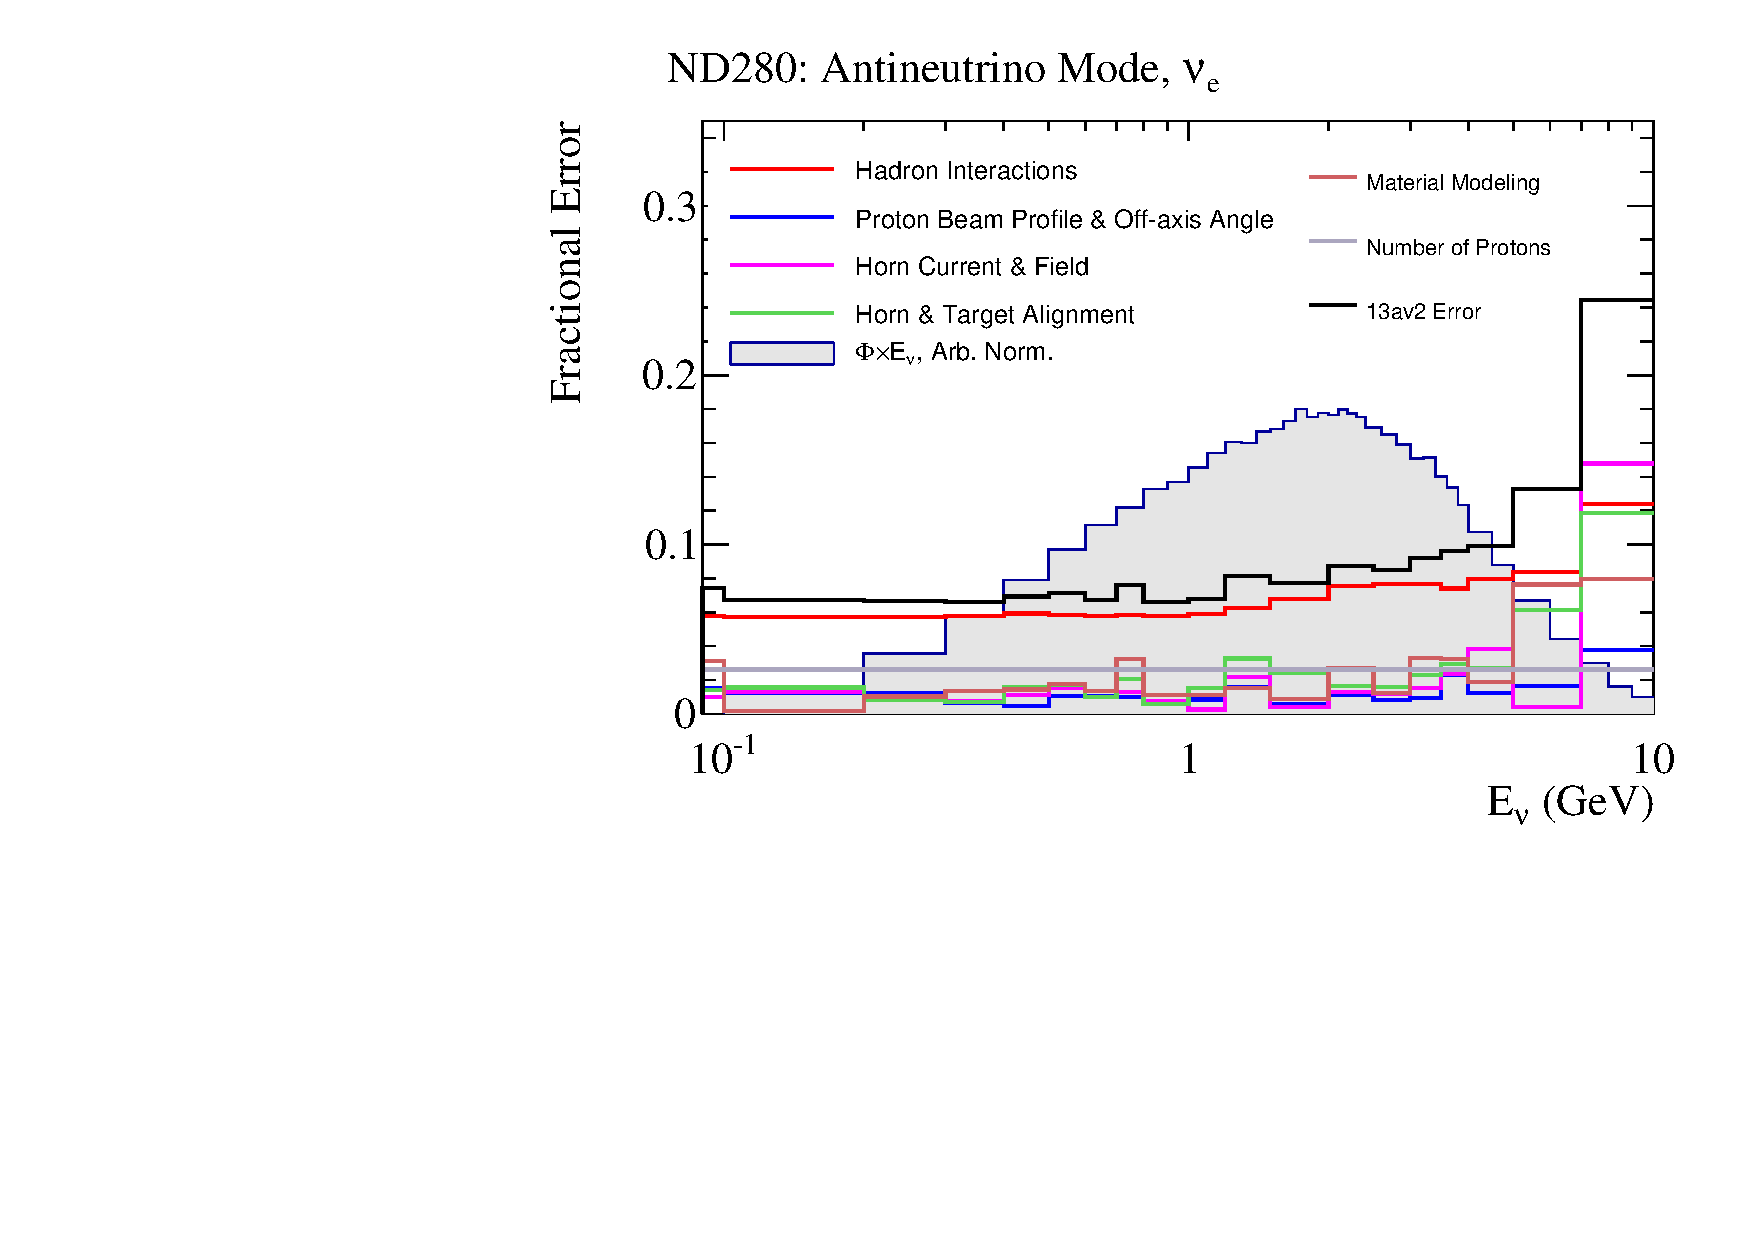
\includegraphics[width=\textwidth, trim={0mm 0mm 0mm 0mm}, clip,page=1]{figures/flux/total_err_nd5_anumode_nue}
	\end{subfigure}
	\begin{subfigure}[t]{0.42\textwidth}
		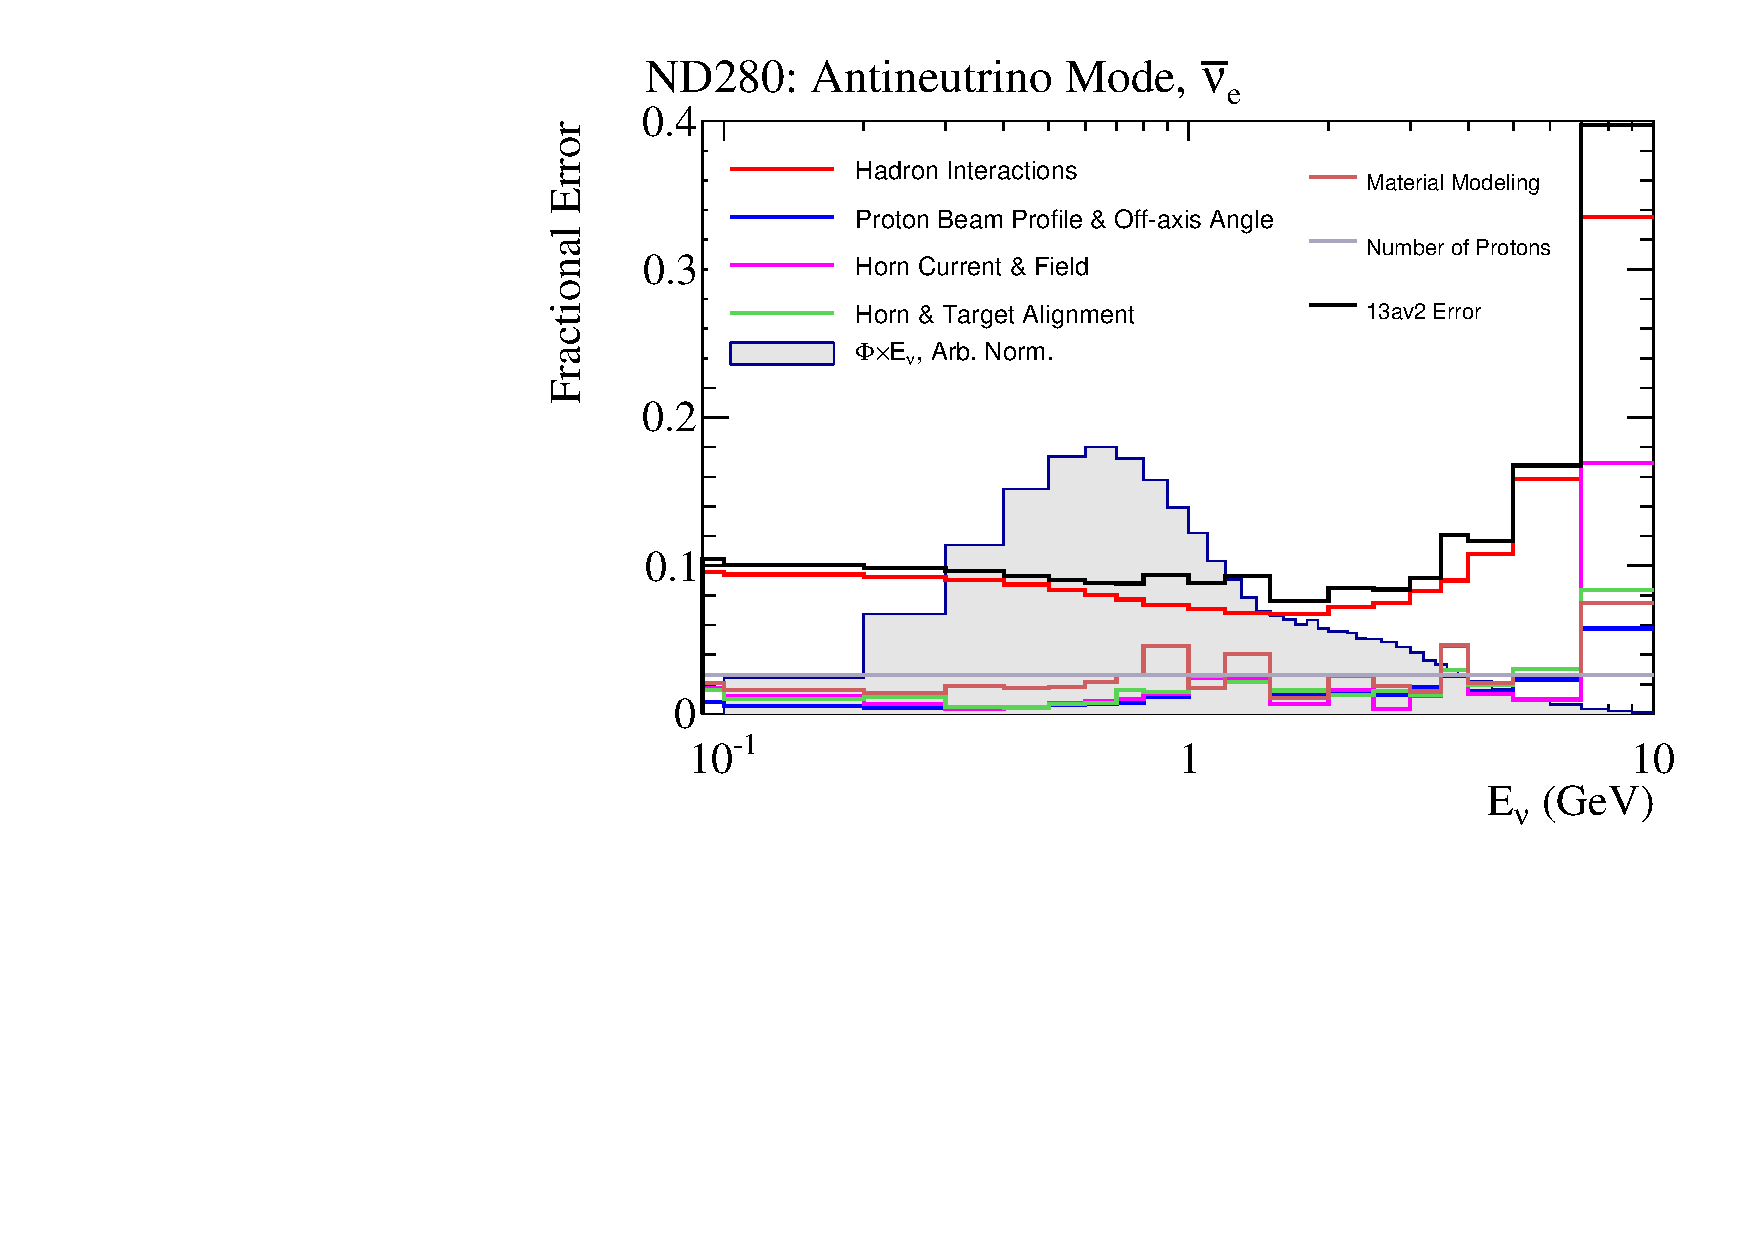
\includegraphics[width=\textwidth, trim={0mm 0mm 0mm 0mm}, clip,page=1]{figures/flux/total_err_nd5_anumode_nueb}
	\end{subfigure}
\caption{RHC flux uncertainties, ``13av2 Error'' is used for this analysis}
\label{fig:flux_uncert_rhc}
\end{figure}

Importantly, the hadronic interaction uncertainty is reducible by improved modelling and tuning to carefully selected relevant hadron production data, which is the main method of reducing the flux uncertainty at T2K. An example of such an effort is the black dashed line and the black solid line in \autoref{fig:flux_uncert_fhc}, which shows the reduction in flux uncertainty from 2014 to 2015 analyses. Additionally, new beam profile monitors aid in reducing the proton beam profile and off-axis angle uncertainties.

The flux systematics enter the near-detector and oscillation analyses as bin-by-bin normalisations in $E_\nu^\text{True}$ for four different neutrino species (\numu, \numubar, \nue, \nuebar), for each running mode (FHC, RHC), for each detector (ND280, SK). The binning is chosen to reflect the magnitude of the neutrino flux and the changing shape but simultaneously keeping the number of parameters relatively low. The right-sign and wrong-sign species have the same binning, so ND280 FHC \numu is binned as ND280 RHC \numubar:
\begin{itemize}
	\item ND280, SK FHC \numu; ND280, SK RHC \numubar, :\\
	$E_\nu^{true}$: 0, 0.4, 0.5, 0.6, 0.7, 1, 1.5, 2.5, 3.5, 5, 7, 30
	
	\item ND280, SK FHC \numubar; ND280, SK RHC \numu:\\
	$E_\nu^{true}$: 0, 0.7, 1, 1.5, 2.5, 30
	
	\item ND280, SK FHC \nue; ND280, SK RHC \nuebar:\\
	$E_\nu^{true}$: 0, 0.5, 0.7, 0.8, 1.5, 2.5, 4, 30
	
	\item ND280, SK FHC \nuebar; ND280, SK RHC \nue:\\
	$E_\nu^{true}$: 0, 2.5, 30
\end{itemize}
This procedure brings the total number of flux parameters to 100: 50 for ND280 and 50 for SK. The SK flux parameters are not directly constrained in the near-detector fit: however because of the very strong ND280-SK flux correlations, the constraint on the ND280 flux parameters from ND280 data indirectly moves SK flux parameters. Hence, all 100 parameters are fit at ND280.

The central values and bin-by-bin uncertainties are highly correlated so the likelihood penalties are evaluated with a covariance matrix, shown in \autoref{fig:flux_cov}.
\begin{figure}[h]
	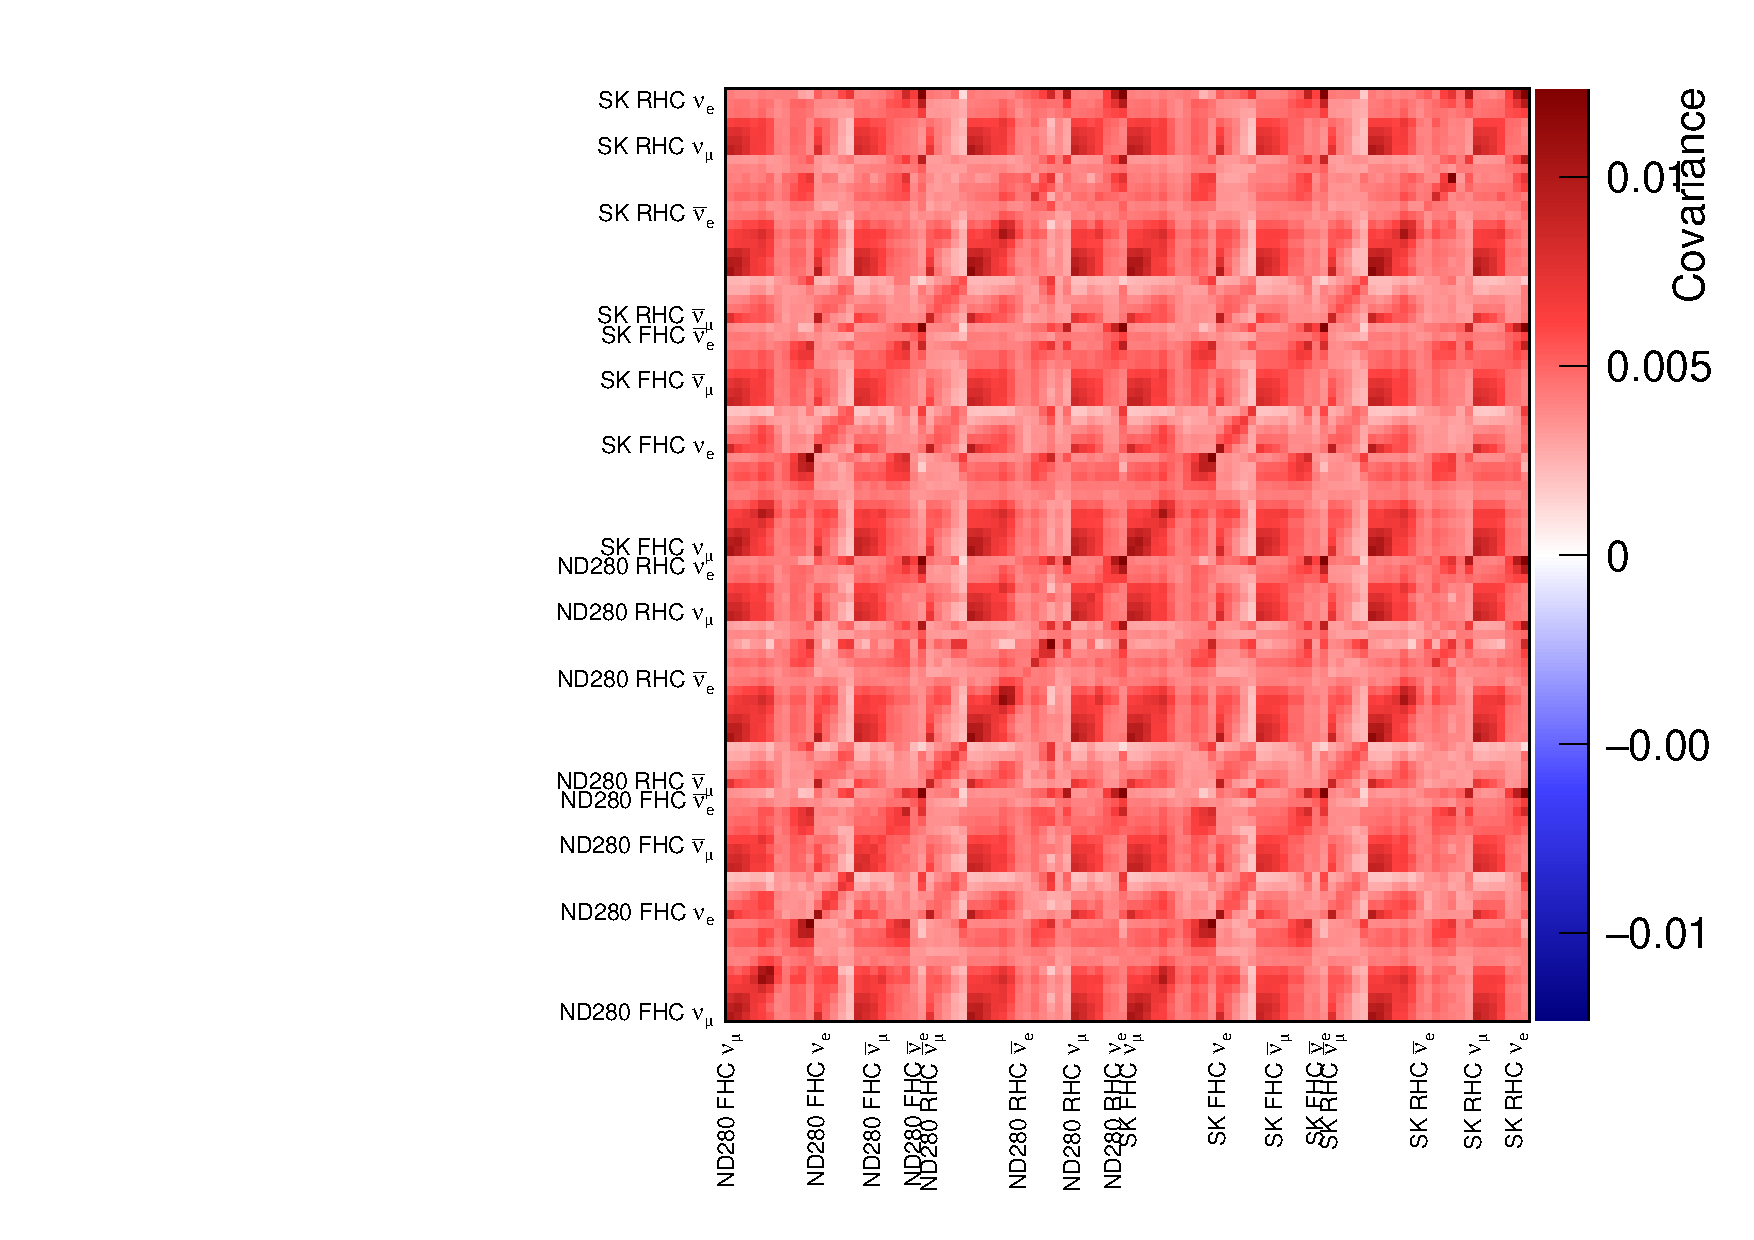
\includegraphics[width=0.45\textwidth, trim={0mm 0mm 0mm 0mm}, clip,page=1]{figures/mach3/inputs/flux_covariance_banff_13av2}
	\caption{13av2 covariance matrix, used in this analysis}
	\label{fig:flux_cov}
\end{figure}

%pi+ to mu+numu 99.9877
%to e+nue 1.23E-4
%Kplus to mu+numu 63.55
%to pi0mu+numu3.353
%to pi0e+nue 5.07
%K0L to pi-mu+numu 27.04
%to pi0e+nue 40.55
%mu+ to e+numubar+nue 100

In addition to the variation systematics above, there is also a nominal flux correction applied to each event as a function of its run period (e.g. run 2a), neutrino specie (e.g. \numubar) and $E_\nu^{\text{True}}$ (e.g. 0.8 GeV). This is present to correct the nominal flux model which the Monte-Carlo was produced with updated measurements. An example from run 4a and run 5b is shown in \autoref{fig:flux_ratio}.
\begin{figure}[h]
	\begin{subfigure}[t]{0.42\textwidth}
		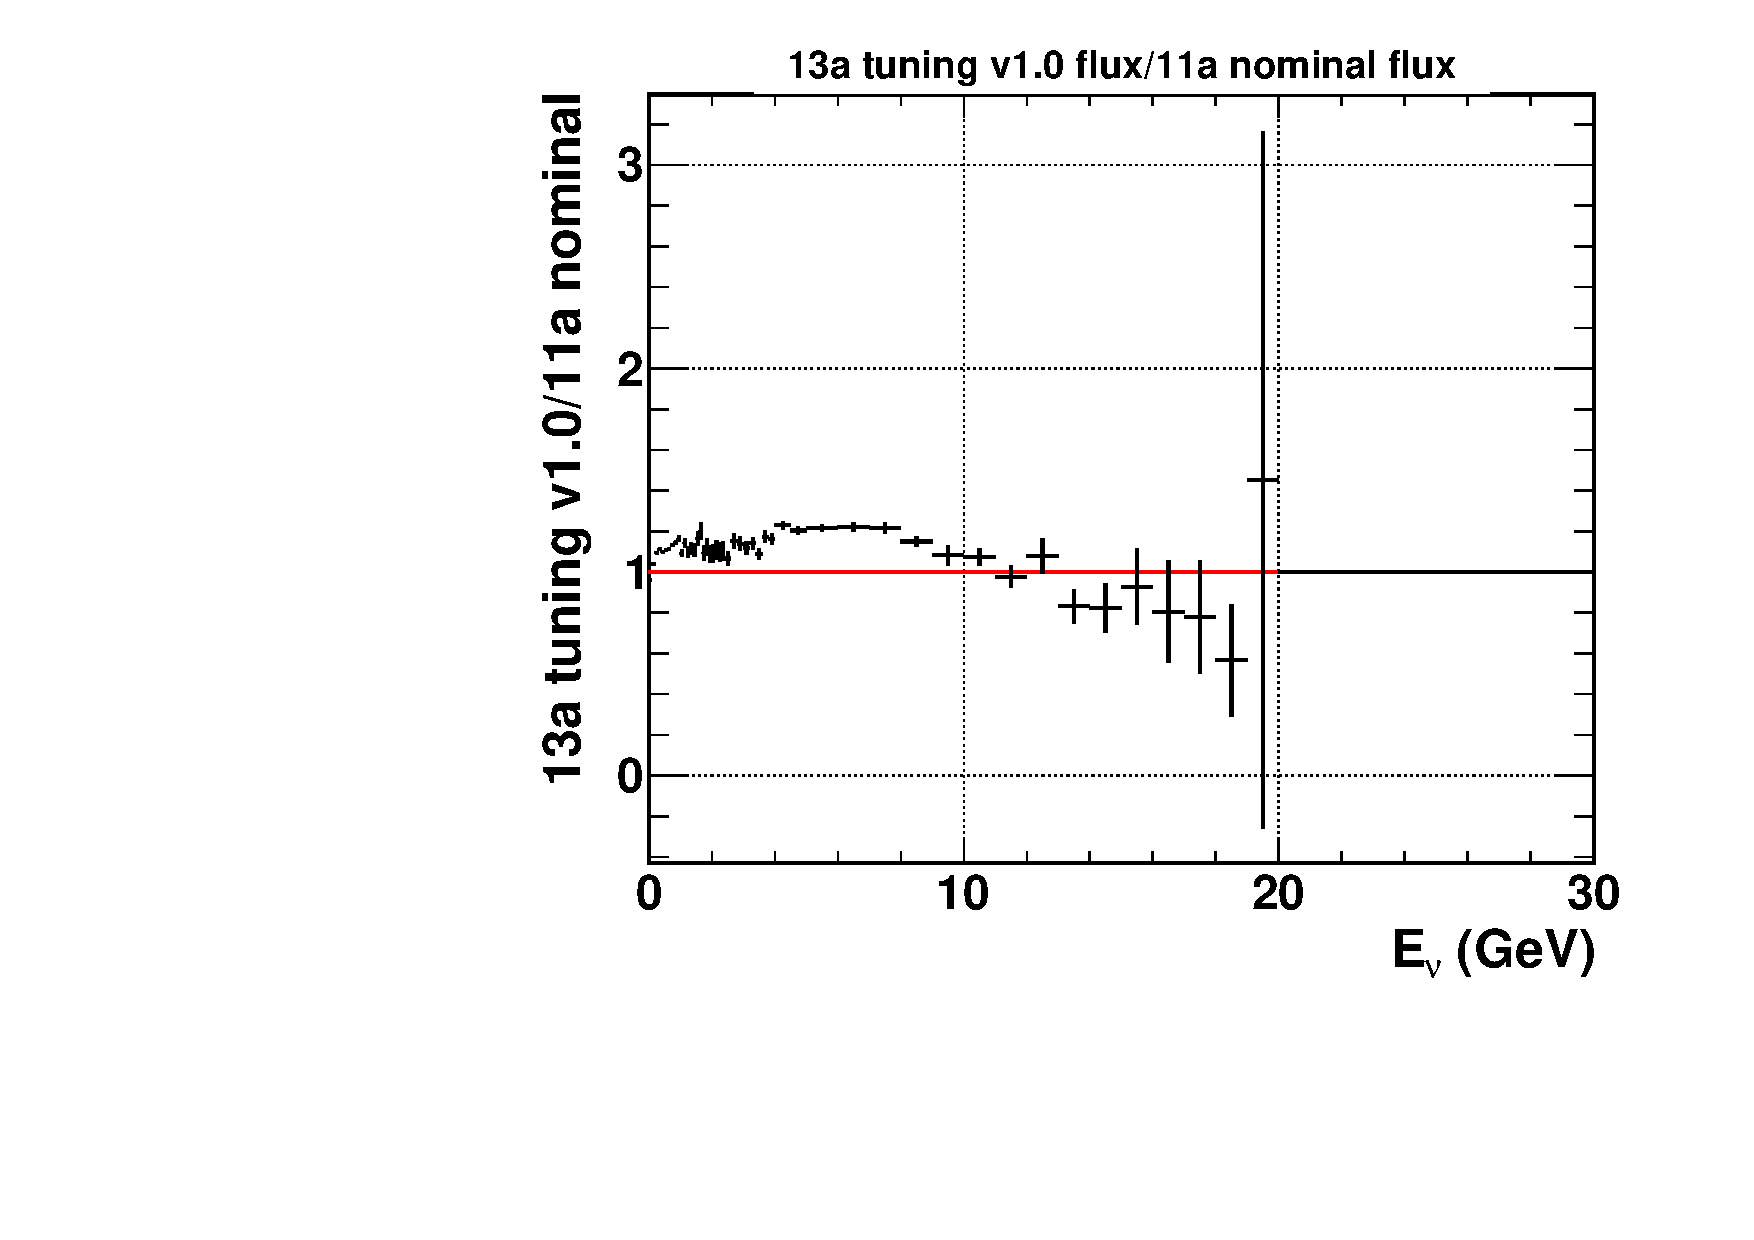
\includegraphics[width=\textwidth, trim={0mm 0mm 0mm 0mm}, clip,page=1]{figures/flux/run4_enu_nd5_13av2_numu_rat}
		\caption{4a \numu}
	\end{subfigure}
	\begin{subfigure}[t]{0.42\textwidth}
		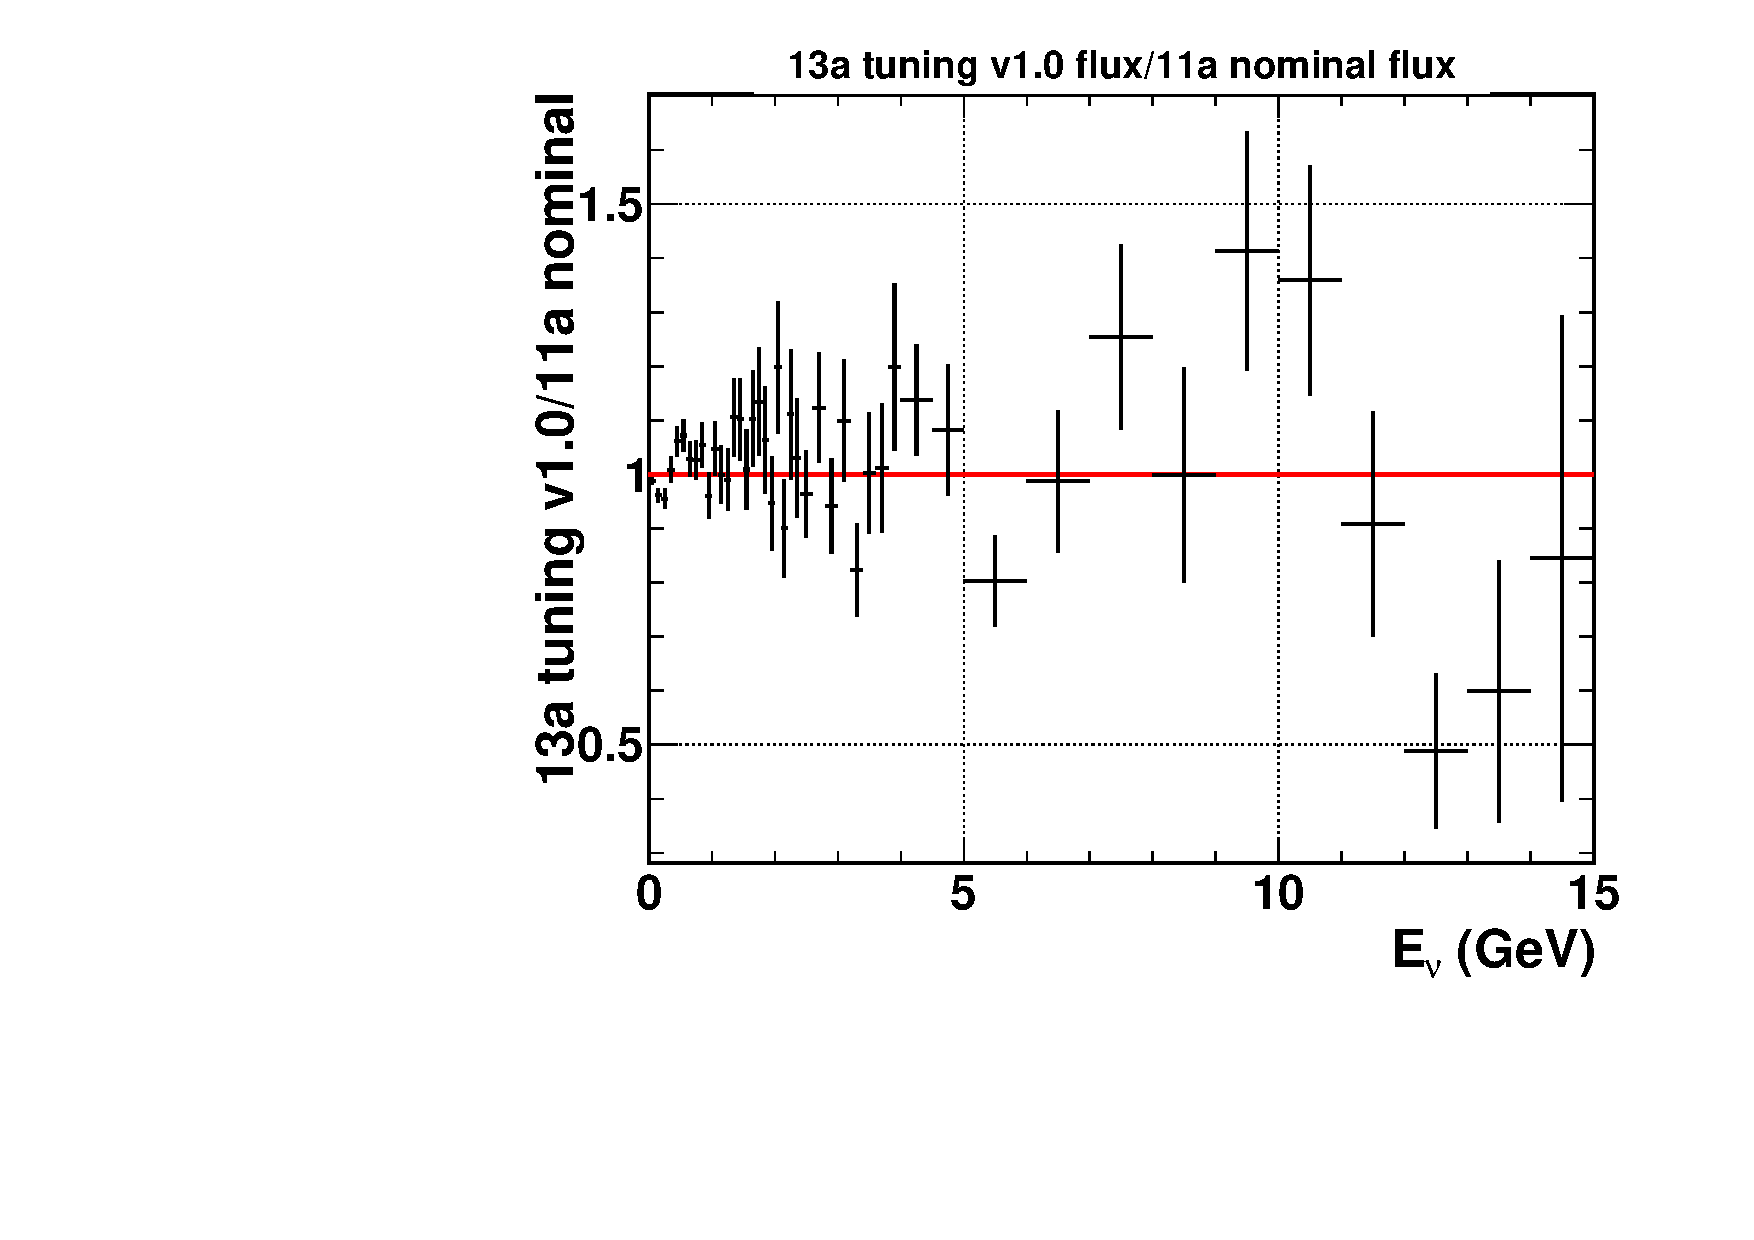
\includegraphics[width=\textwidth, trim={0mm 0mm 0mm 0mm}, clip,page=1]{figures/flux/run5b_enu_nd5_13av2_numubar_rat}
		\caption{5b \numubar}
	\end{subfigure}
	\caption{Nominal flux corrections applied to events in the ND5 tracker plane}
	\label{fig:flux_ratio}
\end{figure}

\subsection{Detector systematics}
\label{subsec:syst_nd280}
The treatment of ND280 detector systematic uncertainties consists of varying the underlying detector systematics, such as TPC PID, FGD PID, TPC Momentum scale and study the impact on the number of predicted events in each \pmu \cosmu bin. 

The parameterisation of near detector systematics are categorised as systematics that purely weight an event as the value changes and systematics that vary the observable event topology. The event weighting can further be broken down into efficiencies (with shapes) and normalisation parameters. When FGD-related systematics are concerned---such as pion tagging by Michel electron identification---the two FGDs have separate implementations to account for geometrical and compositional differences.

The different sources of systematics, their variation type and assumed probability distribution function (PDF) are shown in \autoref{tab:nd280_systs}.
\begin{table}[h]
	\begin{tabular}{l | c c}
	\hline
	\hline
	Systematic						& Variation 	& PDF \\
	\hline
	\multicolumn{3}{l}{TPC} \\
	Magnetic Field Distortions		& Observable 	& Flat \\
	TPC Momentum Scale				& Observable	& Gauss \\
	TPC Momentum Resolution			& Observable	& Gauss \\
	TPC PID							& Observable	& Gauss \\
	TPC Cluster Efficiency			& Efficiency	& Gauss \\
	TPC Tracking Efficiency			& Efficiency	& Gauss \\
	TPC Charge ID Efficiency		& Efficiency	& Gauss \\
	\hline 
	\multicolumn{3}{l}{FGD-TPC} \\
	TPC-FGD Matching Efficiency		& Efficiency	& Gauss \\
	\hline
	\multicolumn{3}{l}{FGD} \\
	FGD PID							& Observable	& Gauss \\
	FGD1-FGD2 Time of Flight		& Observable	& Gauss \\
	FGD Hybrid Tracking Efficiency	& Efficiency	& Gauss \\
	Michel Electron Efficiency		& Efficiency	& Gauss \\
	\hline
	\multicolumn{3}{l}{Backgrounds} \\
	Out-of-Fiducial-Volume			& Normalisation & Gauss \\
	Sand Muons						& Normalisation & Gauss \\
	Pile-Up							& Normalisation	& Gauss \\
	\hline
	\multicolumn{3}{l}{MC modelling} \\
	Pion secondary interactions		& Normalisation & Gauss \\
	FGD Mass						& Normalisation & Gauss \\
	\hline
	\hline
	\end{tabular}
\caption{ND280 systematics present in the fit}
\label{tab:nd280_systs}
\end{table}

\paragraph{Observable variation systematics}
This group of systematics have the potential to change the reconstructed topology, so allow for migration in and out of selections. It can also switch the reconstructed lepton candidate for a different track in the event. The systematic is applied as a smearing to the reconstructed event variables (e.g. \pmu, \cosmu) and then reruns the event selection algorithm on the smeared event.

There are two methods with which the smearing is applied:
\begin{itemize}
	\item If the relevant reconstructed variable has a known true value, the difference between the two is used as a scaling. The updated value of the variable after the variation is then
	\begin{equation}
		x'_{reco} = x_{true} + \left(x_{reco}^{MC}-x_{true}\right)\left(s + \alpha \cdot \delta s\right)
	\end{equation}
	where $\alpha$ is the random variable from the relevant systematic's PDF in \autoref{tab:nd280_systs}, $s$ is the scaling factor, and $\delta s$ is its statistical error. The scaling factor is defined as
	\begin{equation}
		s = \frac{\sigma^{data}}{\sigma^{MC}}
	\end{equation}
	and
	\begin{equation}
		\delta s = s \cdot \left| \frac{\delta \sigma^{data}}{\sigma^{Data}} - \frac{\delta \sigma^{MC}}{\sigma^{MC}} \right|
	\end{equation}
	where $\sigma^{data}$ is the dispersion observed in data and $\delta \sigma^{data}$ is the error on the dispersion.
	\item If the MC is corrected to match a data mean value. This correction is needed because the effect of a systematic error ($\delta \Delta \bar{x}$) on the selected event relative the nominal MC is not guaranteed to agree with the corrected MC. The updated observable is then
	\begin{equation}
		x'_{reco} = x^{MC}_{reco}+ \Delta\bar{x} + \alpha \delta \Delta \bar{x}
	\end{equation}
	where $\Delta\bar{x} = \bar{x}^{data}_{reco}-\bar{x}^{MC}_{reco}$,$\bar{x}_{reco}$ is the mean value of the variable $x$, $\alpha$ is a random variable, and $\delta \Delta \bar{x}$ is the associated uncertainty from the reconstructed data and MC discrepancy,
	\begin{equation}
		\delta \Delta \bar{x} = \sqrt{\Delta\bar{x}^2 + \left(\delta \bar{x}^{data}_{reco}\right)^2  + \left(\delta \bar{x}^{MC}_{reco}\right)^2}
	\end{equation}
\end{itemize}

Additionally uncertainties from the magnetic field has special cases of the above:
\begin{itemize}
	\item The TPC laser calibration corrections are used on-top of the B-field mapping corrections, where the latter is applied during reconstruction and the former is treated as an uncertainty. The reconstructed variable is then
	\begin{equation}
		x'_{reco} = x^{MC}_{reco} + \alpha \left(x_{reco}^{New}-x_{reco}^MC\right)
	\end{equation}
	where $\alpha$ is the random variable and $x_{reco}^{New}$ is the reconstructed momentum after the updated mapping is applied. This applies to the magnetic field distortion systematic.
	\item If the observable depends on a scale $s$ that is easy to extract from in-situ measurements
	\begin{equation}
		x'_{reco} = x_{reco}^{MC}+\alpha \delta x
	\end{equation}
	where $\delta x = x_{reco}^{MC} \delta s$ is the uncertainty on the observable and $\delta s$ is the uncertainty on the scaling variable. The TPC momentum scale systematic uses this parameterisation, in which $s$ is the scale of the magnet current and $\delta s$ is its uncertainty.
\end{itemize}

\paragraph{Efficiency systematics}
The weight systematics are computed from studies which compare data and MC predictions in well known control samples. The multiple ND280 subdetectors enable cross-checks for tracking and matching efficiencies: e.g. TPC2 tracking efficiency can be computed using tracks with segments in FGD1 and FGD2, which therefore should have a track in TPC2.

Using the sand muon control sample---defined as having a through-going muon track in most of the detector, where the muon was created in the surrounding sand in the ND280 pit or the magnet---as an example, such muons tend to be very forward-going and high energy. Thus the sample is suitable for alignment studies but not efficiency (since the \pmu, \cosmu phase space is very limited). The model assumed to move to this phase space assumes the ratio between efficiencies in data and MC are the same in analysis and control samples.

The efficiency using MC is calculated using the truth information and the calculated efficiency for the data is then
\begin{equation}
\epsilon_{data} = \frac{\epsilon_{data}^{Control}}{\epsilon_{MC}^{Control}} \epsilon_{MC}
\end{equation}
where $\epsilon^{Control}$ is the efficiency in the control sample(s). The statistical uncertainty in $r^{Control} = \epsilon^{Control}_{data}/\epsilon^{Control}_{MC}$ is taken into account as
\begin{equation}
\delta r^{Control} = \sqrt{\left(1-r^{Control}\right)^2 + \left(\delta r^{Control}_{Stat}\right)^2}
\end{equation}
yielding the predicted efficiency in the data as
\begin{equation}
\epsilon_{data}' = \left(r^{Control} + \alpha \delta r^{Control}\right)\epsilon_{MC}
\end{equation}
where $\alpha$ is the random variable.

Finally to propagate the weight systematics on an event-by-event basis we define the two weights
\begin{equation}
w_{Eff} = \frac{\epsilon_{data}'}{\epsilon_{MC}}
\end{equation}
for events that identify the track correctly and
\begin{equation}
w_{Ineff} = \frac{1-\epsilon_{Data}'}{1-\epsilon_{MC}}
\end{equation}

\paragraph{Normalisation systematics}
These systematics are simple one-time weights which change the overall event numbers. The FGD mass error is an example of such a systematics: if the mass of the FGD is larger than the nominal, the overall number of observed events in MC should be increased. The weight $w$ is simple applied as
\begin{equation}
w = 1+\alpha \cdot \delta e
\end{equation}
where 1.0 is the nominal weight, $\alpha$ is a random variable, and $\delta e$ is the systematic error on the source.

\red{talk about all the detector systematics in summary?}

\paragraph{Relative systematic error sizes}
\autoref{tab:nd280_syst_error_nu} shows the relative errors from ND280 systematics contribution on the number of predicted events for the different ND280 \numu selections for FGD1. The total error for the CC0$\pi$ selection is 1.66\%, CC1$\pi$ is 3.33\% and CCOther 6.47\%. For comparison, the flux and cross-section errors are generally $\mathcal{O}\left(10\%\right)$. The error increases with selection because the increased track multiplicity and lower ``cleanliness'' of the reconstructed events. 

The largest contribution to the total error is pion secondary interactions, making up $\sim90\%$ of the detector systematics. This systematic additionally has the power to migrate events through selections by changing the number of reconstructed pions. For the CCOther selection the TPC tracking efficiency also has a large contribution (1.79\%), decreasing to 0.44\% for CC1$\pi$ and 0.27\% for CC0$\pi$. The FGD mass contributes a 0.6\% uncertainty for all selections, making up 1/3 of the error on CC0$\pi$ selection.
\begin{table}[h]
	\begin{tabular}{l | c c c}
		\hline
		\hline
		Systematic & \multicolumn{3}{c}{Percentage error} \\
				   & CC0$\pi$ & CC1$\pi$ & CCOther \\ 
		\hline	
		\multicolumn{4}{l}{TPC} \\
		Magnetic Field Distortions		& 0.025 & 0.063 & 0.072 \\
		TPC Momentum Scale				& 0.062 & 0.074 & 0.230 \\
		TPC Momentum Resolution			& 0.055 & 0.094 & 0.286 \\
		TPC PID							& 0.316 & 0.792 & 0.616 \\
		TPC Cluster Efficiency			& 0.000 & 0.000 & 0.002 \\
		TPC Tracking Efficiency			& 0.259 & 0.440 & 1.786 \\
		TPC Charge ID Efficiency		& 0.178 & 0.270 & 0.473 \\
		\hline 
		\multicolumn{4}{l}{FGD-TPC} \\
		TPC-FGD Matching Efficiency		& 0.148 & 0.270 & 0.605 \\
		\hline
		\multicolumn{4}{l}{FGD} \\
		FGD PID							& 0.011 & 0.034 & 0.015 \\
		FGD1-FGD2 Time of Flight		& 0.034 & 0.070 & 0.017 \\
		FGD Hybrid Tracking Efficiency	& 0.106 & 0.100 & 0.532 \\
		Michel Electron Efficiency		& 0.062 & 0.253 & 0.008 \\
		\hline
		\multicolumn{4}{l}{Backgrounds} \\
		Out-of-Fiducial-Volume			& 0.391 & 0.541 & 0.286 \\
		Sand Muons						& 0.069 & 0.085 & 0.031 \\
		Pile-Up							& 0.112 & 0.112 & 0.112 \\
		\hline
		\multicolumn{4}{l}{MC modelling} \\
		Pion secondary interactions		& 1.433 & 3.173 & 6.118 \\
		FGD Mass						& 0.595 & 0.595 & 0.595 \\
		\hline
		Total & 1.660 & 3.329 & 6.467 \\
		\hline
		\hline
	\end{tabular}
\caption{Integrated systematic errors for FGD1 FHC related systematics}
\label{tab:nd280_syst_error_nu}
\end{table}
FGD2 has similarly sized systematic contributions, although slightly modified due to the ND280 geometry, e.g. the sand muon error is smaller in FGD2 due to tighter vetos than in FGD1.

\autoref{tab:nd280_syst_error_nubar} shows the same table but for the RHC selections. The tracking related systematics for the FGD (Michel electron tagging, PID, hybrid tracking) are not present because the number of tracks in the event---defining the 1Trk or NTrk selection---is solely based on the number of TPC tracks present, so has no impact.

As for the FHC selections, the largest systematic by far is the pion secondary modelling (90+\%). The impact is larger than for FHC selections since the source of pions are \numu interactions (typically higher in $E_\nu$ so also higher in multiplicity) and the larger uncertainties on $\pi^-$ re-interaction probabilities. The FGD mass is again the second largest systematic for CC0$\pi$, although for the CCNTrk selection the TPC tracking efficiency comes in second, followed by the TPC PID, followed by the FGD mass.
\begin{table}[h]
	\begin{tabular}{l | c c}
		\hline
		\hline
		Systematic & \multicolumn{2}{c}{Percentage error} \\
				   & CC1Trk & CCNTrk \\ 
		\hline	
		\multicolumn{3}{l}{TPC} \\
		Magnetic Field Distortions		& 0.004 & 0.165 \\
		TPC Momentum Scale				& 0.049 & 0.246 \\
		TPC Momentum Resolution			& 0.041 & 0.123 \\
		TPC PID							& 0.307 & 0.544 \\
		TPC Cluster Efficiency			& 0.000 & 0.002 \\
		TPC Tracking Efficiency			& 0.436 & 1.201 \\
		TPC Charge ID Efficiency		& 0.117 & 0.115 \\
		\hline 
		\multicolumn{3}{l}{FGD-TPC} \\
		TPC-FGD Matching Efficiency		& 0.109 & 0.394 \\
		\hline
		\multicolumn{3}{l}{FGD} \\
		FGD1-FGD2 Time of Flight		& 0.016 & 0.009 \\
		\hline
		\multicolumn{3}{l}{Backgrounds} \\
		Out-of-Fiducial-Volume			& 0.336 & 0.610 \\
		Sand Muons						& 0.153 & 0.248 \\
		Pile-Up							& 0.240 & 0.241 \\
		\hline
		\multicolumn{3}{l}{MC modelling} \\
		Pion secondary interactions		& 4.902 & 9.198 \\
		FGD Mass						& 0.598 & 0.584 \\
		\hline
		Total 							& 5.371 & 10.378 \\
		\hline
		\hline
	\end{tabular}
	\caption{Integrated systematic errors for FGD1 RHC related systematics}
	\label{tab:nd280_syst_error_nubar}
\end{table}

\paragraph{Parameterisation of ND280 related systematics}
The systematics in \autoref{tab:nd280_systs} could theoretically be varied on an event-by-event basis. However, in practice this is complicated by two main reasons: 1) the event selection framework is not sufficiently optimised to guarantee fast reweighting below 0.1s per reconfigure; 2) and for some events and values of variation systematics, discontinuous test-statistic were found when events were migrated from one topology to another. Whereas the former is purely computational, the latter causes problems for finding minima with gradient descent algorithms, employed by the dedicated near-detector only fit (BANFF). 

It was instead decided to parameterise the systematics similarly to the flux systematics, which both ensures smoothness and enables fast reweighting. The systematics listed in \autoref{tab:nd280_systs} are varied on an event-by-event and 500 random variations are chosen according to the prior covariances and the number of events are binned in the chosen fit-binning in \autoref{sec:binning_2017}. Each bin is then a normalisation parameter, and highly correlated with adjacent bins through a covariance matrix. Finally, an MC statistical covariance matrix and a covariance matrix shifting the MC reconstructed lepton momentum of CCQE events by 20 MeV to roughly emulate the effects from Martini-Nieves 1p1h model\red{cite} differences are added. The central value and uncertainty on the number of events in a bin comes from a the arithmetic mean and the central value is the rms, and a cross-check with a Gaussian fit is done.

\begin{figure}[h]
	\begin{subfigure}[t]{0.42\textwidth}
		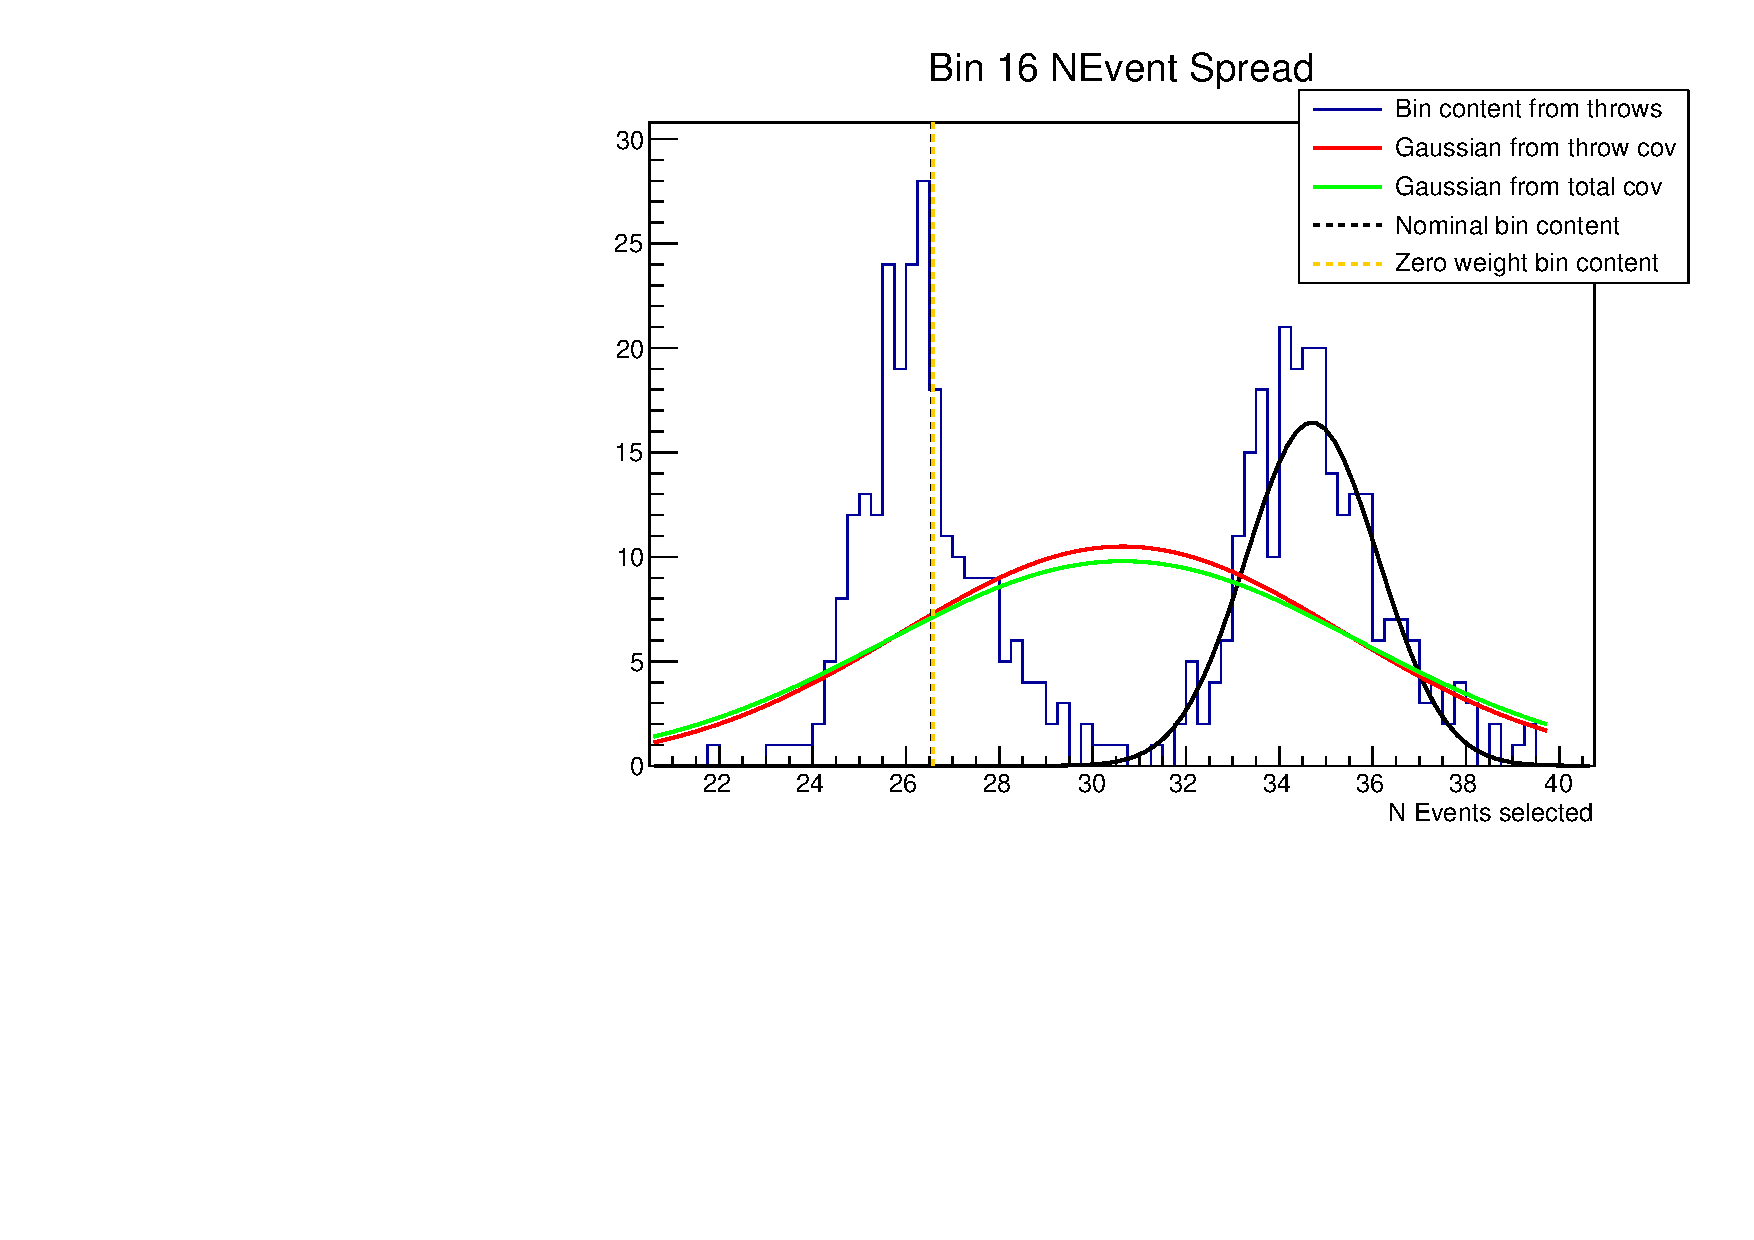
\includegraphics[width=\textwidth, trim={4mm 3mm 2mm 2mm}, clip,page=1]{figures/numu/syst/bad_bin}
		\caption{FGD1 CC0$\pi$, 1250-2000, 0.6-0.7}
	\end{subfigure}
	\begin{subfigure}[t]{0.42\textwidth}
		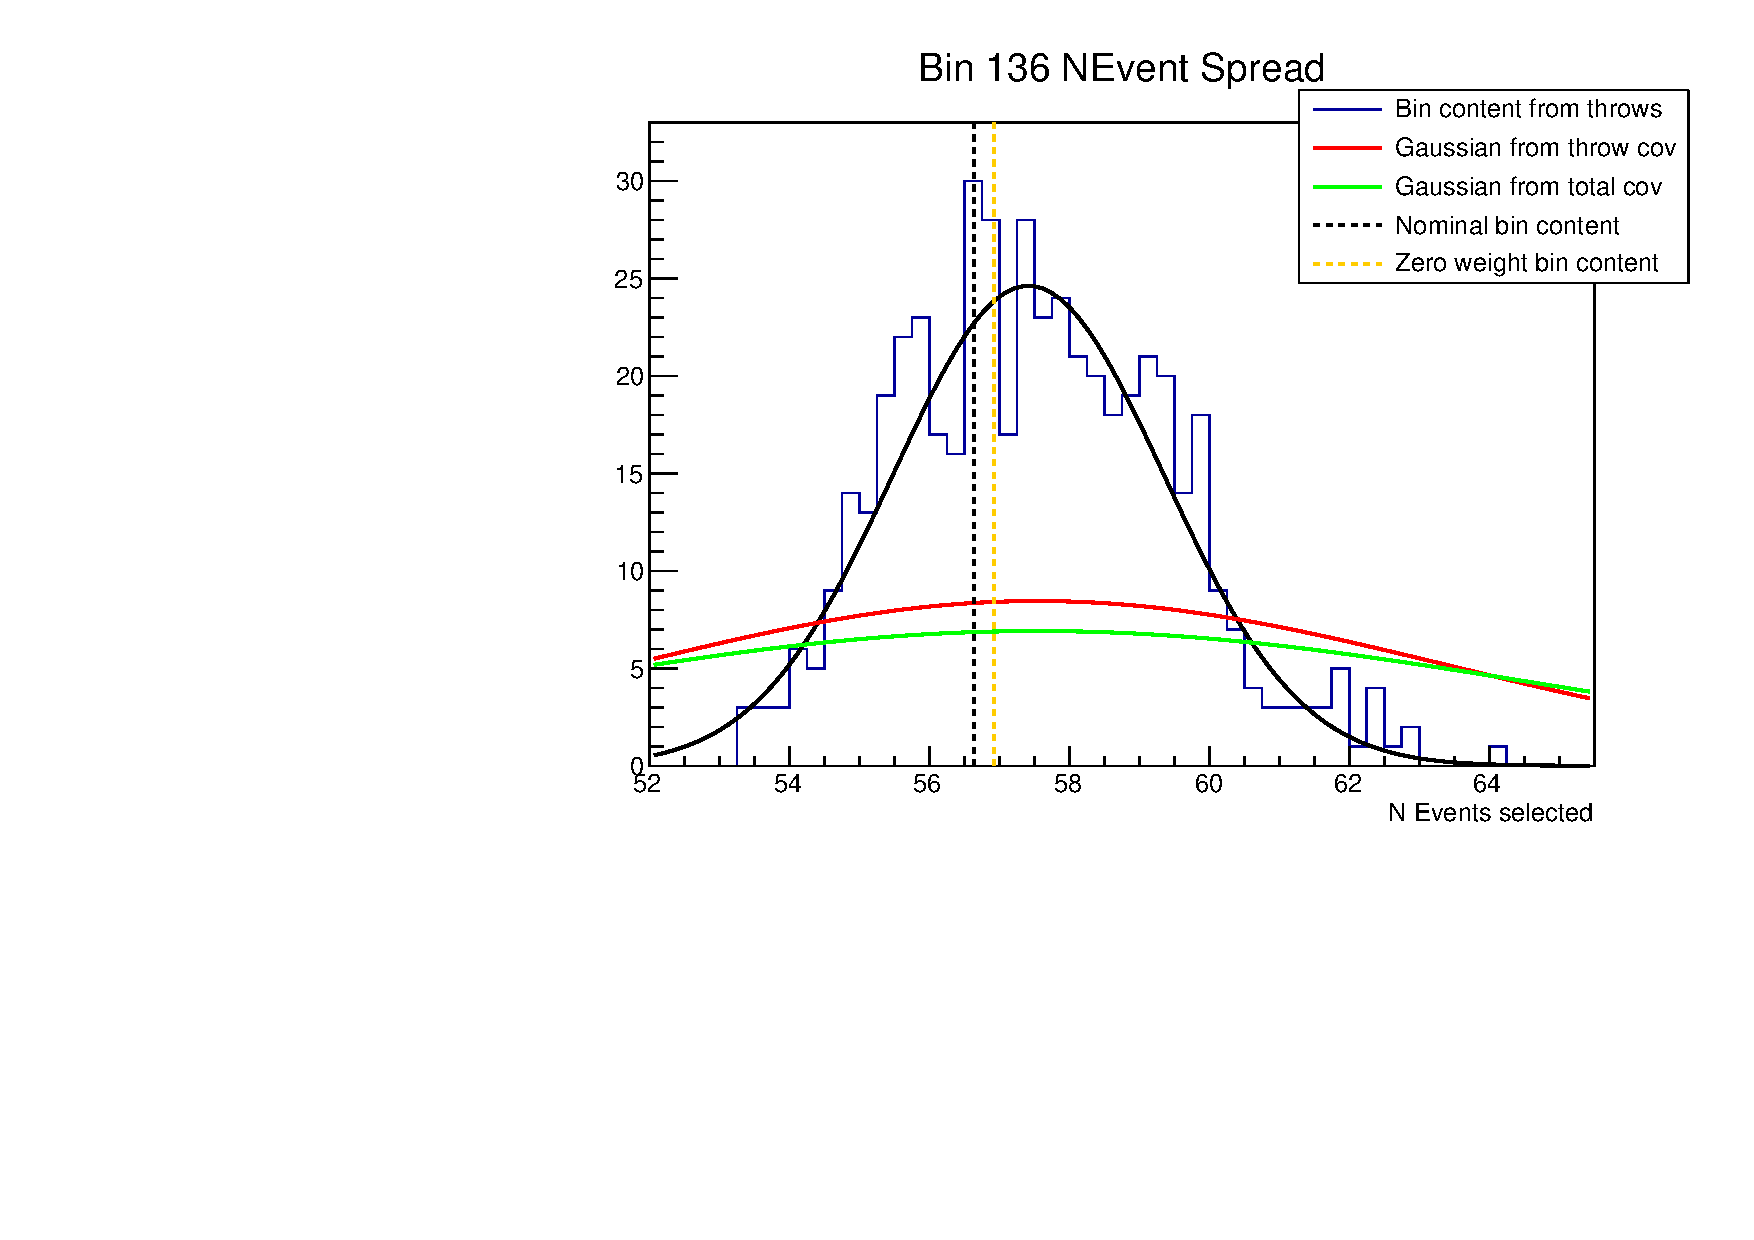
\includegraphics[width=\textwidth, trim={4mm 3mm 2mm 2mm}, clip,page=1]{figures/numu/syst/decent_bin}
		\caption{FGD1 CC1Trk, 0-400, 0.97-0.98}
	\end{subfigure}

	\begin{subfigure}[t]{0.42\textwidth}
		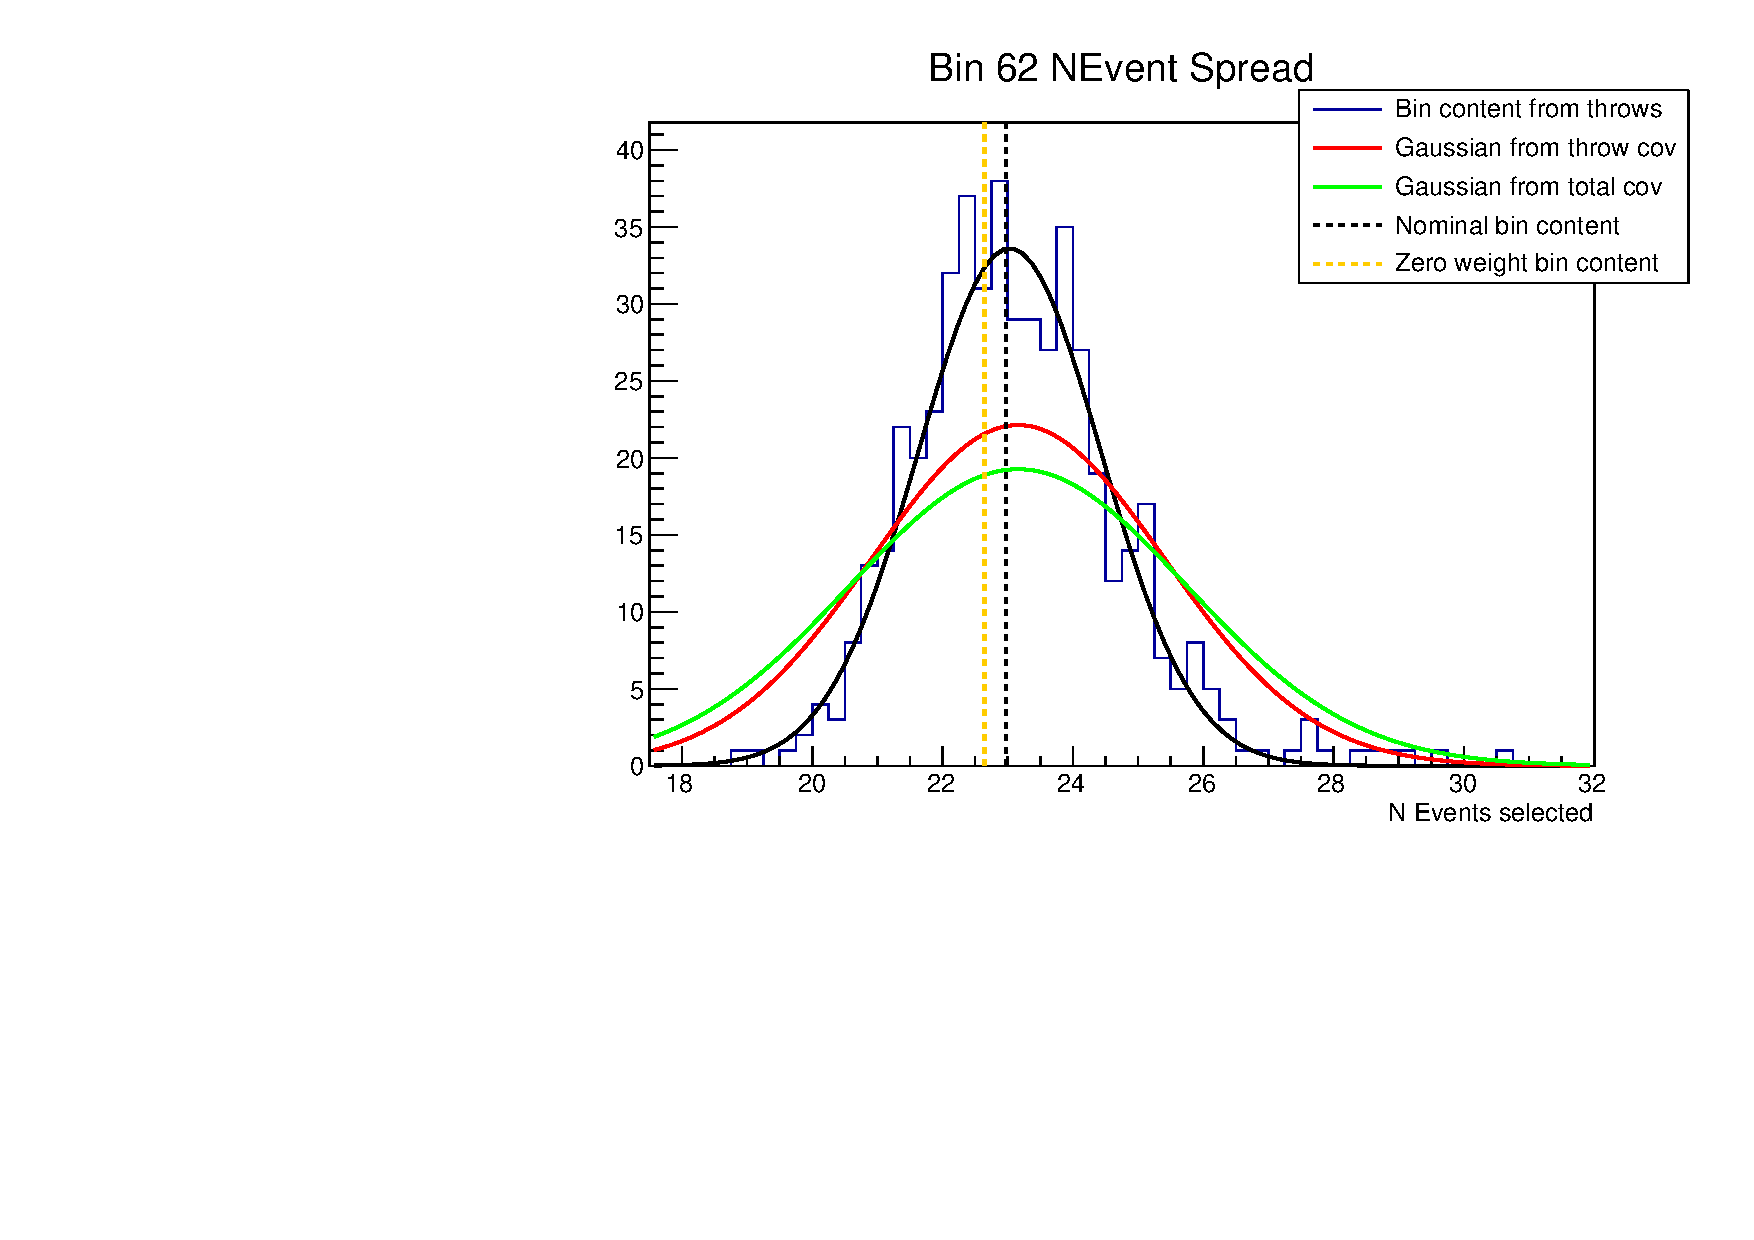
\includegraphics[width=\textwidth, trim={4mm 3mm 2mm 2mm}, clip,page=1]{figures/numu/syst/good_bin}
		\caption{FGD1 CC1$\pi$, 300-1250, 0.9-0.92}
	\end{subfigure}
	\begin{subfigure}[t]{0.42\textwidth}
		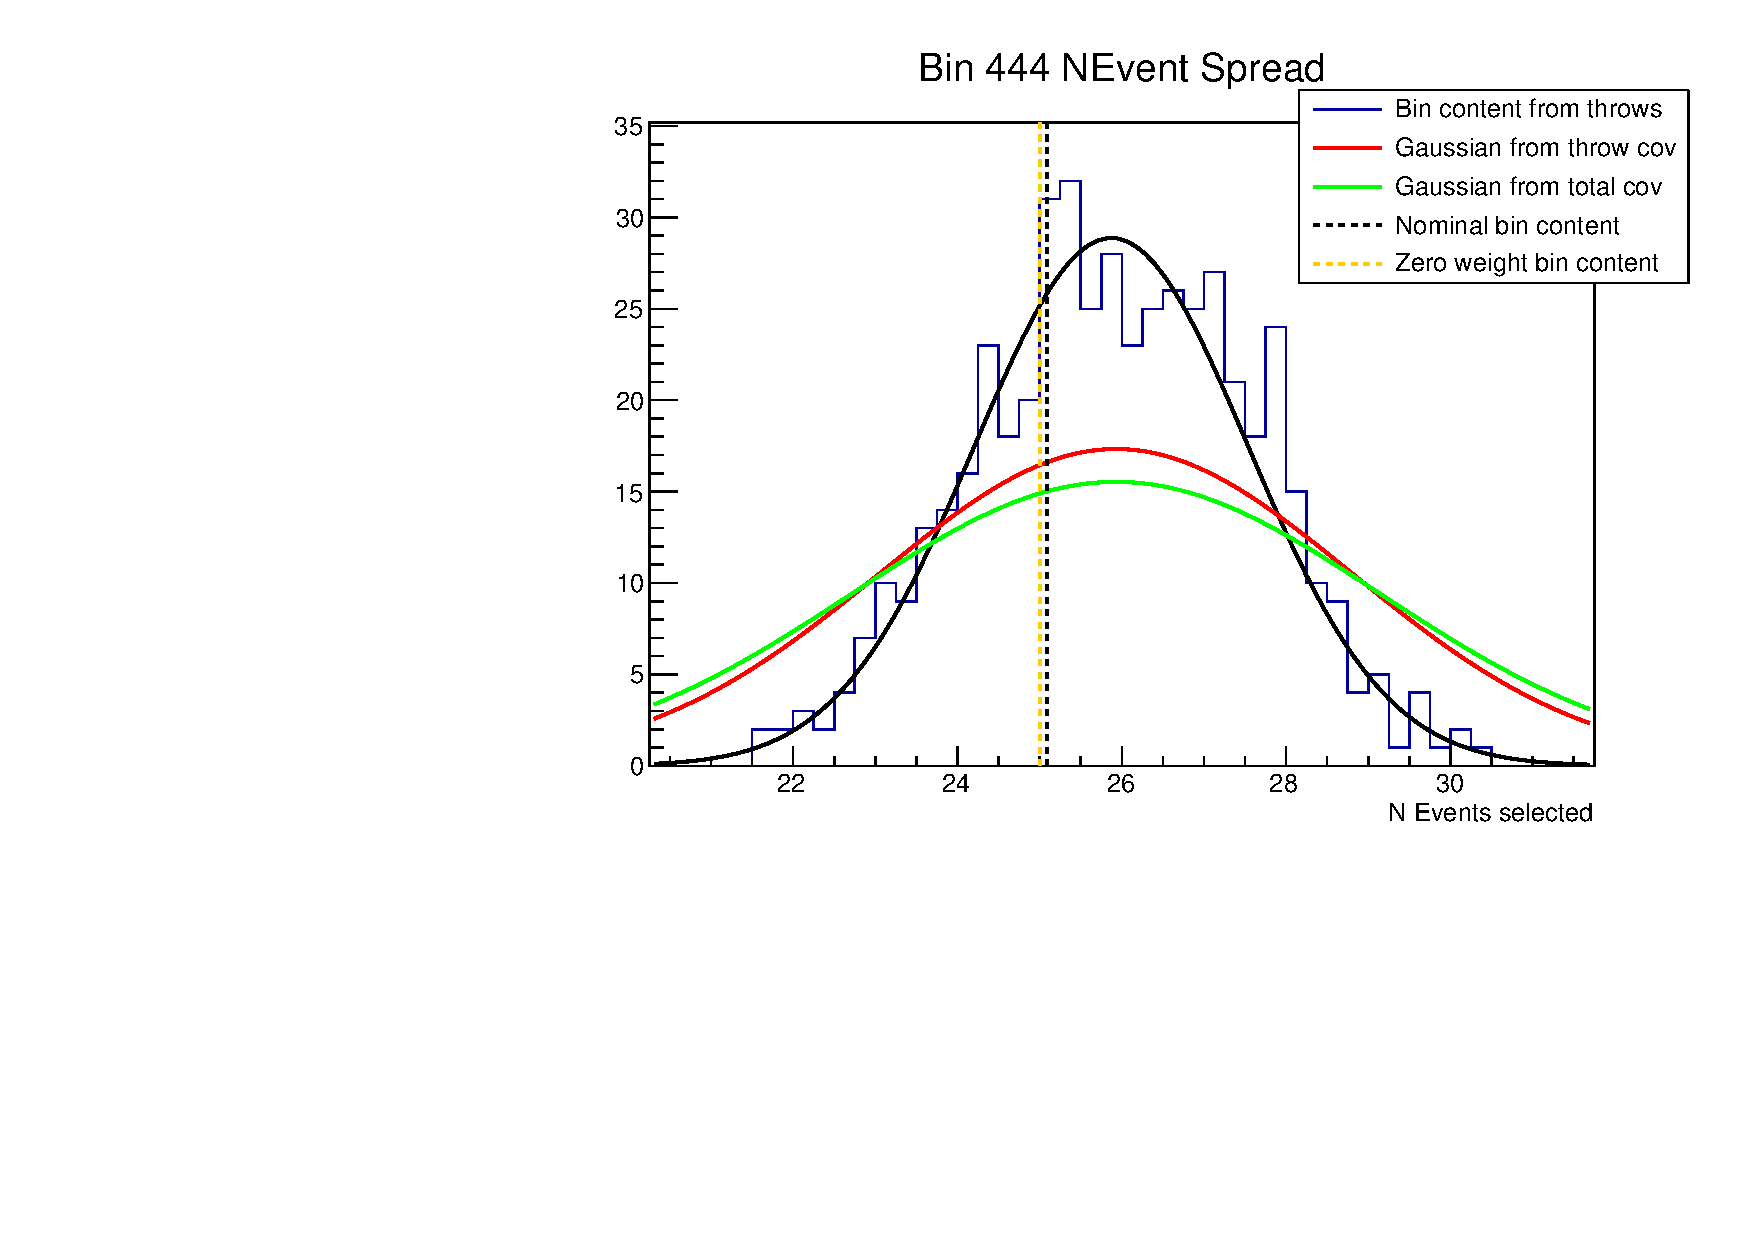
\includegraphics[width=\textwidth, trim={4mm 3mm 2mm 2mm}, clip,page=1]{figures/numu/syst/good_bin2}
		\caption{FGD2 CCNTrk, 0-700, 0.93-0.98}
	\end{subfigure}
	\caption{Number of events in selected detector bins with uncertainties from ND280 systematics}
	\label{fig:det_var}
\end{figure}
The result of the detector systematics procedure is shown in \autoref{fig:det_var} for a selection of bins. In FGD1 CC0$\pi$ we note a particularly bad fit to the \pmu=1250-2000, \cosmu=0.6-0.7 bin, in which we see a double Gaussian bimodal behaviour, likely from event migrating in and out of the sample due to pion secondary interactions. Although a simple fit to the bin content chooses one of the peaks, the covariance matrix entry sits in between the two with an error that covers both modes.

%see TN 212 p 95
%read p39 onwards about syst

\begin{figure}[h]
	\begin{subfigure}[t]{0.70\textwidth}
		\includegraphics[width=\textwidth, trim={0mm 0mm 0mm 0mm}, clip,page=1]{figures/numu/syst/nd280_syst_cov.pdf}
	\end{subfigure}
\end{figure}

\begin{figure}[h]
	\begin{subfigure}[t]{0.70\textwidth}
		\includegraphics[width=\textwidth, trim={0mm 0mm 0mm 0mm}, clip,page=2]{figures/numu/syst/nd280_syst_cov.pdf}
	\end{subfigure}
\end{figure}

The number of detector systematics still decreased slightly from 580 to 556 due to merging bins with similar detector systematic effects for the rebinned samples.
All the consecutive bins with similar systematic values have been merged in order to reach a lower number of parameters (556) while the number of bins in the fit increased a lot (1624 bins), keeping the number of parameters under control.
It has been demonstrated with Asimov fits, the results of which are shown in \autoref{fig:2017_rebin_asimov}, that the effect of this rebinning was small.

The effect of changing the ND280 systematics binning was done with an older cross-section model than which the fit was completed in. This was due to a late delivery of the cross-section model \red{write an appendix on this model}. The flux parameters were entirely consistent.
\begin{table}
	\centering
	\begin{tabular}{ l | c | c }
		\hline
		Parameter & Fit binning & Similar syst. merge \\
		\hline
		\hline
		FSI INEL LO & $0.0 \pm 0.202$ & $0.0\pm0.200$ \\
		FSI INEL HI & $0.0 \pm 0.235$ & $0.0\pm0.233$ \\
		FSI PI PROD & $0.0 \pm 0.347$ & $0.0\pm0.344$ \\
		FSI CEX LO  & $0.0 \pm 0.416$ & $0.0\pm0.412$ \\
		FSI CEX HI  & $0.0 \pm 0.193$ & $0.0\pm0.191$ \\
		$M_A^{QE}$  & $1.2 \pm 0.0517$ & $1.2\pm0.0512$ \\
		$p_F^{C}$   & $217 \pm 36.96$ & $217\pm36.021$ \\
		2p2h norm C & $100 \pm 30.79$ & $100\pm30.56$ \\
		$E_B^{C}$   & $25.0 \pm 8.57$ & $25.0\pm8.56$ \\
		$p_F^{O}$   & $225 \pm 57.61$  & $225\pm56.16$ \\
		2p2h norm O & $100 \pm 277.98$ & $0.0\pm272.62$ \\
		$E_B^{C}$   & $27.0 \pm 9.00$ & $27.0\pm9.00$ \\
		$C_5^A$		& $1.01 \pm 0.066$ & $1.01\pm0.064$ \\
		$M_A^{1\pi}$ & $0.95 \pm 0.060$ & $0.95\pm0.059$ \\
		$I_{1/2}$ non-res & $1.30 \pm 0.180$ & $1.30\pm0.180$ \\
		CC $\nu_e$ norm & $1.00 \pm 0.030$ & $1.00\pm0.030$ \\
		DIS Shape	& $0.00 \pm 0.208$ & $0.0\pm0.208$ \\
		CC Coherent norm & $1.0 \pm 0.258$ & $1.0\pm0.257$ \\
		NC Coherent norm & $1.0 \pm 0.299$ & $1.0\pm0.299$ \\
		NC Other & $1.0 \pm 0.182$ & $1.0\pm0.181$ \\
		2p2h $\bar{\nu}$ & $1.0 \pm 0.332$ & $1.0\pm0.329$ \\
		\hline
	\end{tabular}
	\caption{Cross-section parameter results from comparisons using fit binning and a merged binning for the 2015 cross-section model.}
\label{fig:2017_rebin_asimov}
\end{table}

The merged systematics binning was improved to:
\begin{itemize}
	\item FHC $\nu_{\mu}$~CC0$\pi$ bin edges: \\
	\pmu (MeV/c): 0, 1000, 1250, 2000, 3000, 5000, 30000 \\
	\cosmu:  -1, 0.6, 0.7, 0.8, 0.85,0.94, 0.96, 1
	\item FHC $\nu_{\mu}$~CC1$\pi$  bin edges: \\
	\pmu (MeV/c):  0, 300, 1250, 1500, 5000, 30000 \\
	\cosmu: -1, 0.7, 0.85, 0.9, 0.92, 0.96, 0.98, 0.99, 1
	\item FHC $\nu_{\mu}$~CCOther bin edges: \\
	\pmu (MeV/c): 0, 1500, 2000, 3000, 5000, 30000 \\
	\cosmu:  -1, 0.8, 0.85, 0.9, 0.92, 0.96, 0.98, 0.99, 1
	\item RHC $\bar{\nu}_{\mu}$~CC 1-Track bin edges: \\
	\pmu (MeV/c): 0, 400, 900, 1100, 2000, 10000 \\
	\cosmu:  -1, 0.6, 0.7, 0.88, 0.95, 0.97, 0.98, 0.99, 1.00
	\item RHC $\bar{\nu}_{\mu}$~CC N-Track bin edges: \\
	\pmu (MeV/c):  0, 700, 1200, 1500, 2000, 3000, 10000 \\
	\cosmu: -1, 0.85, 0.88, 0.93, 0.98, 0.99, 1.00
	\item RHC $\nu_{\mu}$~CC 1-Track bin edges: \\
	\pmu (MeV/c):  0, 400, 800, 1100, 2000, 10000 \\
	\cosmu:   -1, 0.7, 0.85, 0.90, 0.93, 0.96, 0.98, 0.99, 1.00
	\item RHC $\nu_{\mu}$~CC N-Track bin edges: \\
	\pmu (MeV/c):  0, 1000, 1500, 2000, 3000, 10000 \\
	\cosmu: -1, 0.8, 0.90, 0.93, 0.95, 0.96, 0.97, 0.99, 1.00
\end{itemize}
Be mega clear that each of these above make up one parameter

\subsection{Cross-section}
\label{subsec:syst_xsec}
splines vs normalisation parameter, Maybe extra bit on BeRPA because of involvement
